 % !TEX program = xelatex
% !TEX encoding = UTF-8 Unicode
\documentclass[12pt,a4paper,zihao=-4,AutoFakeBold,AutoFakeSlant,fontset=fandol]{ctexart}
\usepackage{iftex}
\usepackage{xeCJK}
\xeCJKsetup{CJKecglue={}}  % 关闭中英文自动间距
\usepackage{amsmath,amsthm,amssymb,amsfonts,mathrsfs,mathtools}
\usepackage{graphicx,caption,float}
\usepackage{geometry,fancyhdr}
\usepackage{enumerate}
\usepackage{tablefootnote}
\usepackage{tocloft}
\usepackage[colorlinks,linkcolor=black,anchorcolor=black,citecolor=black]{hyperref}
\usepackage[symbol]{footmisc}
\usepackage{cleveref}
\usepackage{fontspec}
\usepackage{setspace}
\usepackage{framed}
\usepackage{mdframed}
\usepackage{array}
\usepackage{booktabs}
\usepackage{tabularx}
\usepackage{xcolor}
\usepackage[boxed,ruled,lined,linesnumbered]{algorithm2e}
\usepackage{algorithmic}
\usepackage{listings,lstautogobble}
\usepackage{appendix}
\usepackage{unicode-math}
\usepackage{multirow}

% 当前环境缺少小标宋字体，使用系统宋体作为稳定替代，避免字体探测触发交互提示。
\newcommand\xiaobiaosong{\songti}

% 上标引用格式
\makeatletter
\def\@cite#1#2{\textsuperscript{[{#1\if@tempswa , #2\fi}]}}
\makeatother

% 统一排版参数
\setstretch{2.0}
\setlength{\parindent}{2em}
\setlength{\parskip}{0pt}

% 页面格式
\geometry{left=3.17cm,right=3.17cm,top=2.54cm,bottom=2.54cm}
\setlength{\headheight}{15pt}

% 目录和正文的页眉与页脚
\fancypagestyle{plain}
 {\fancyhf{}
  \fancyfoot[C]{\zihao{-5}\thepage}
  \renewcommand\headrulewidth{0pt}
  \renewcommand\footrulewidth{0pt}}
\fancypagestyle{body}
 {\fancyhf{}
  \fancyfoot[C]{\zihao{-5}\thepage}
  \fancyhead[C]{\zihao{-4}金融反诈智能守护赛题一作品技术文档}
  \renewcommand\headrulewidth{0.6pt}
  \renewcommand\footrulewidth{0pt}}

% 设置图和表格全文连续编号
\renewcommand{\thefigure}{\arabic{figure}}
\renewcommand{\thetable}{\arabic{table}}

% 图表题注分隔符：编号与题名之间空两格
\DeclareCaptionLabelSeparator{twospaces}{\hspace{2em}}

% 自定义 caption 字体：小四号宋体
\DeclareCaptionFont{songtixiaosi}{\songti\zihao{-4}}

\captionsetup[figure]{
  font=songtixiaosi,
  labelfont=songtixiaosi,
  labelsep=twospaces,
  justification=centering,
  singlelinecheck=true,
  name=图
}

\captionsetup[table]{
  font=songtixiaosi,
  labelfont=songtixiaosi,
  labelsep=twospaces,
  justification=centering,
  singlelinecheck=true,
  name=表
}

% 图表标题使用中文
\AtBeginDocument{%
  \renewcommand{\figurename}{图}
  \renewcommand{\tablename}{表}
  \renewcommand{\refname}{\centering\heiti\zihao{4}参考文献}
  \renewcommand{\contentsname}{\centering\heiti\zihao{4}目\quad 录}
  \renewcommand{\appendixname}{附录}
}

% 标题格式与编号层级
\renewcommand\thesection{\chinese{section}、}
\renewcommand\thesubsection{（\chinese{subsection}）}
\renewcommand\thesubsubsection{\arabic{subsubsection}.}
\ctexset{
  section = {
    format = \heiti\zihao{-3}\raggedright,
    numberformat = {},
    aftername = {},
    beforeskip = 24pt,
    afterskip = 12pt
  },
  subsection = {
    format = \kaishu\zihao{4}\raggedright,
    numberformat = {},
    aftername = {},
    beforeskip = 12pt,
    afterskip = 6pt
  },
  subsubsection = {
    format = \songti\zihao{-4}\bfseries\raggedright,
    numberformat = {},
    aftername = {},
    beforeskip = 12pt,
    afterskip = 6pt
  }
}

% Configure cleveref to use Chinese names
\crefname{figure}{图}{图}
\crefname{table}{表}{表}
\crefname{section}{第}{节}
\crefname{appendix}{附录}{附录}

\begin{document}

\pagestyle{empty}

\begin{titlepage}
\centering

\vspace*{0.3cm}

{\heiti\zihao{3}作品编号：\underline{\makebox[6cm][c]{}}}

\vspace{2.2cm}

{\xiaobiaosong\fontsize{20pt}{24pt}\selectfont\bfseries 2026睿抗机器人开发者大赛}

\vspace{0.6cm}

{\xiaobiaosong\zihao{1}\bfseries CAIP强脑赛道参赛作品}

\vspace{0.9cm}

{\heiti\zihao{4}金融反诈智能守护\quad 赛题一：欺诈交易智能识别}

\vspace{1.8cm}

{\xiaobiaosong\zihao{3}\bfseries FP-FraudSim流式欺诈交易智能识别系统}

\vspace{3cm}

{\zihao{-2}
\renewcommand\arraystretch{2.2}
\begin{center}
  {\heiti 参赛队伍：}\fangsong\underline{\makebox[7cm][c]{}}\\
  {\heiti 作品方向：}\fangsong\underline{\makebox[7cm][c]{欺诈交易智能识别}}\\
  {\heiti 提交日期：}\fangsong\underline{\makebox[7cm][c]{2026年6月}}
\end{center}
}

\vfill

{\fangsong\zihao{-2} 2026年6月}

\end{titlepage}


\clearpage
\pagenumbering{Roman}
\setcounter{page}{1}
\pagestyle{plain}
\begin{sloppypar}
  \section*{\centering\heiti\zihao{4}摘\quad 要}
\addcontentsline{toc}{section}{摘要}

\vspace{0.5cm}

{\zihao{-4}
面向金融反诈智能守护赛题一“欺诈交易智能识别”的要求，本文档给出FP-FraudSim流式风控系统的完整技术方案与工程实现说明。系统围绕第三方支付跨时段、跨渠道交易风险防控场景，构建从仿真数据生成、欺诈模式注入、流式实时识别、风险等级输出、团伙溯源分析到人工反馈迭代的端到端闭环，目标是在交易发生时完成低延迟风险评分，并为人工研判提供可解释证据。

系统采用Kafka + Flink + Redis + FastAPI + Dashboard的工程架构。离线侧通过公开交易仿真数据规范化与场景注入，构造账户接管、钓鱼转账、洗钱拆分、卡农账户、优惠滥用、商户套现、设备团伙欺诈等七类样本；训练侧融合用户画像、设备指纹、IP环境、商户行为、短时窗口统计和图关联特征，支持LightGBM、XGBoost、CatBoost、sklearn等多模型训练与排行榜管理；在线侧由Flink消费交易流，实时计算5分钟、10分钟、1小时窗口特征，从Redis补齐画像和图风险，调用模型服务输出风险分数、风险等级、处置动作与理由码，并将结果写入risk\_results、alert\_events和late\_events等主题。

围绕赛题评分准则，系统重点实现四项能力：一是可重复的多源异构仿真环境与跨渠道交易流回放；二是Kafka + Flink微批评分链路与批量推理接口，兼顾吞吐和延迟；三是人工反馈与轻量重训机制，支持新增欺诈样本回流和模型热切换；四是基于共享设备、IP、商户、收款方的图挖掘模块，输出疑似团伙、风险得分和证据链。工程层面提供Docker Compose编排、一键启动脚本、API压测脚本、单元测试与可视化看板，便于初赛复现和现场答辩演示。

本文档的贡献在于将赛题一要求拆解为可运行系统模块，并在文档中逐项对齐完成度、创新性、实用性、成熟度和安全性评分点。系统不是单一离线分类模型，而是具备交易仿真、实时检测、动态异常识别、可解释溯源和持续迭代能力的金融反诈原型。
}

\vspace{0.6cm}

\noindent{\heiti\zihao{-4}关键词：}{\zihao{-4}金融反诈；欺诈交易识别；Kafka；Flink；图挖掘；模型迭代}

\end{sloppypar}

\newpage
\begingroup
\setcounter{tocdepth}{3}
\setstretch{1.35}
\setlength{\cftbeforesecskip}{2pt}
\setlength{\cftbeforesubsecskip}{0.5pt}
\setlength{\cftsubsubsecnumwidth}{1.5em}
\tableofcontents
\endgroup

\clearpage
\setcounter{page}{1}
\pagenumbering{arabic}
\pagestyle{body}

\vspace{0.5\baselineskip}

\section{赛题理解与总体目标}
\label{sec:intro}

\subsection{赛题一任务拆解}

赛题一“欺诈交易智能识别”面向金融交易全链路风险防控场景，要求参赛团队自建或模拟多源异构交易环境，并在交易发生时完成实时风险评估、欺诈判定和风险等级输出。其目标不是单纯训练一个二分类模型，而是形成覆盖数据仿真、实时计算、模型识别、风险解释和持续迭代的完整反诈系统。

结合规则文件，赛题一的核心交付可以拆解为以下六类能力：

\begin{enumerate}
  \item \textbf{仿真环境：}模拟用户、账户、商户、设备、IP、渠道、支付方式等对象，生成正常交易与多类型欺诈交易，体现跨时段和跨渠道行为；
  \item \textbf{实时检测：}将交易组织为流式输入，建立数据接入、画像补齐、窗口特征计算、模型推断、风险输出的在线链路；
  \item \textbf{多维特征：}融合用户行为、设备指纹、IP环境、商户画像、短时交易窗口、交易网络和图挖掘特征；
  \item \textbf{模型迭代：}支持多模型训练、阈值校准、人工反馈样本回流、轻量重训和在线模型热切换；
  \item \textbf{团伙识别：}基于共享设备、共享IP、共同收款方和高风险商户挖掘疑似欺诈团伙，并输出可解释证据；
  \item \textbf{工程落地：}提供可部署架构、性能测试方案、监控看板、测试用例和安全合规设计。
\end{enumerate}

\subsection{作品定位}

本作品命名为FP-FraudSim流式风控系统，定位为面向第三方支付和互联网金融交易的实时欺诈识别原型。系统以“仿真交易流 + 流式风险计算 + 模型服务 + 图谱溯源 + 人工反馈”为主线，覆盖赛题一完成度评分中的四个明确子项：仿真环境与实时检测能力、流式数据处理框架、自适应学习与模型迭代能力、多维度特征构建。

与只提交离线Notebook或静态分类结果的方案相比，本系统强调三个工程闭环。第一，数据闭环：通过ETL、七类欺诈注入脚本与可调参数仿真器生成可复现实验流，再由Producer按速率回放至Kafka。第二，识别闭环：Flink计算窗口特征并调用模型服务，风险结果实时进入Kafka主题和Dashboard。第三，迭代闭环：人工复核标签同时写入反馈主题和样本池，训练脚本生成候选模型，经指标对比后受控发布，并保留快速回滚版本。

\subsection{问题驱动的技术路线}

金融交易反诈具有\textbf{风险发生快、欺诈样本少、行为关系复杂、业务误报成本高、欺诈手法持续变化}等特点。因此，技术路线不能只追求离线分类精度，而需要同时解决实时性、识别效果、可解释性和持续迭代问题。

\begin{enumerate}
  \item \textbf{针对“事后识别来不及”的问题，选择Kafka + Flink流式架构。}Kafka将交易接入与风险计算解耦，可缓冲流量峰值并支持结果回放；Flink面向有状态流计算，能够按事件时间维护用户、设备和商户窗口，并通过watermark处理乱序交易。这比定时批处理更适合在支付发生时完成风险判定。
  \item \textbf{针对“单笔交易看似正常”的问题，构建画像、窗口与图关联多维特征。}用户历史画像用于判断行为偏离，短时窗口用于识别爆发式异常，设备/IP和图关联用于发现多账户协同关系，使系统从单笔静态判断升级为跨时段、跨实体研判。
  \item \textbf{针对“结构化数据、类别特征多且样本不均衡”的问题，选择梯度提升模型作为主模型。}LightGBM、XGBoost和CatBoost能够有效处理非线性特征交互、缺失值及类别变量，在中等规模表格数据上训练和推理成本较低；系统以PR-AUC、Top 1\%召回和误报率评价模型，更符合低欺诈率业务场景。
  \item \textbf{针对“团伙欺诈难以由单笔模型发现”的问题，引入可解释图挖掘和GraphSAGE旁路实验。}共享资源与连通分量方法负责稳定产出证据链；GraphSAGE验证图嵌入价值，但不直接影响线上主模型，兼顾创新性与稳定性。
  \item \textbf{针对“黑盒结果难以直接处置”的问题，输出理由码并提供阈值沙盒。}模型分数被映射为放行、复核和拒绝决策，评审或业务人员可调整两级阈值，实时观察精度、召回、误拦和审核工作量变化。
  \item \textbf{针对“欺诈模式持续漂移”的问题，设计受控模型生命周期。}人工反馈进入样本池后生成candidate候选模型，经评估后提升为latest，旧模型自动备份为rollback，避免反馈驱动重训直接覆盖线上模型。
\end{enumerate}

\subsection{评分准则对应关系}

表~\ref{tab:score_mapping}按照赛题一评分细则拆分系统能力，并列出评审时可以直接核验的交付证据。后文按照该映射展开技术实现、实验验证和安全设计。

\begin{table}[H]
  \centering
  \caption{赛题评分点与系统实现对应关系}
  \label{tab:score_mapping}
  \renewcommand\arraystretch{1.3}
  \setlength{\tabcolsep}{3pt}
  {\songti\zihao{5}
  \begin{tabularx}{0.98\textwidth}{>{\raggedright\arraybackslash}p{1.45cm}>{\centering\arraybackslash}p{0.7cm}>{\raggedright\arraybackslash}X>{\raggedright\arraybackslash}X}
    \toprule
    评分项 & 分值 & 核心实现 & 可核验交付证据 \\
    \midrule
    仿真与实时检测 & 5 & 七类场景注入、可调参数仿真、交易流回放与风险分级 & 仿真配置、Producer、实时结果与告警界面 \\
    流式处理框架 & 5 & Kafka接入、Flink事件时间与窗口计算、迟到事件分流 & Docker服务、Flink UI、风险/告警/迟到主题 \\
    自适应学习与迭代 & 5 & 反馈样本池、candidate/latest/rollback、阈值沙盒 & 反馈接口、候选指标、发布/回滚与重载接口 \\
    多维特征构建 & 5 & 交易、画像、设备/IP、窗口、商户和图关联特征 & 特征配置、窗口代码、Redis画像、图特征产物 \\
    创新性 & 20 & 微批评分、图证据、GraphSAGE旁路、阈值沙盒 & 图实验指标、证据图、阈值交互、一键演示 \\
    实用性 & 20 & 风险处置、接口接入、边云部署与性能验证 & API输出、Dashboard、Compose/K8s清单、压测报告 \\
    成熟度 & 20 & 模块化、多模型适配、测试覆盖、受控模型生命周期 & 单元测试、版本产物、发布回滚接口、技术文档 \\
    安全性 & 20 & API Key、双通道审计、Secret与网络隔离 & audit日志/主题、K8s Secret、NetworkPolicy、安全方案 \\
    \midrule
    技术作品项合计 & 100 & 覆盖完成度、创新性、实用性、成熟度和安全性 & 由系统演示、代码工程、测试结果和本文档共同证明 \\
    \bottomrule
  \end{tabularx}
  }
\end{table}

\noindent\textbf{说明：}团队表现为额外10分加分项，主要通过答辩逻辑、现场协作和问题应答体现，不计入表~\ref{tab:score_mapping}所列技术作品项100分。

\subsection{文档结构}

本文档第二节说明数据仿真、欺诈场景和特征体系；第三节介绍系统架构、实时处理链路、模型训练、图挖掘和可视化交互；第四节给出实验验证、性能测试方案与复现流程；第五节总结创新点、应用价值、安全合规和后续优化方向。

\section{需求流程与数据分析}
\label{sec:data}

\subsection{需求场景及诈骗行为特征分析}

正常交易通常具有稳定的设备、IP、时间、金额和收款习惯；诈骗交易则常表现为陌生设备登录、金额突然偏离、短时高频、多账户共享资源、资金集中流向高风险收款方等异常。系统据此将业务需求转换为“事件接入、实时特征提取、多证据融合、双阈值处置、证据链溯源、人工反馈迭代”六个连续步骤，并以低风险放行、中风险复核和高风险拦截作为最终业务输出。

\begin{figure}[H]
  \centering
  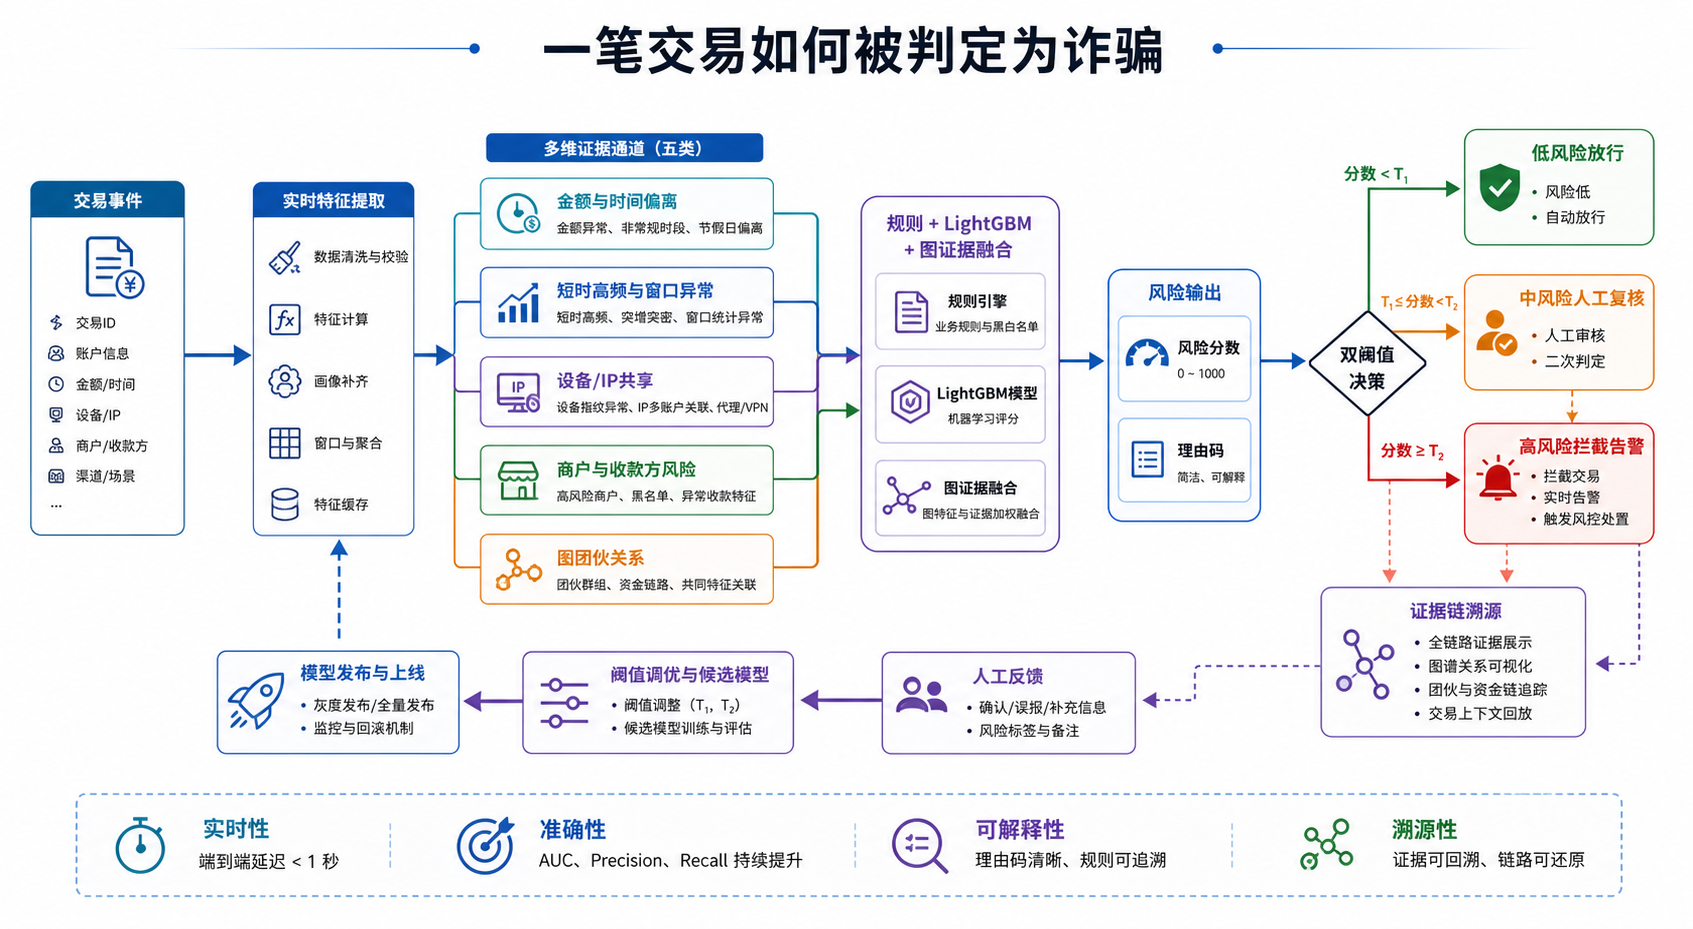
\includegraphics[width=0.98\textwidth]{pic/fraud_decision_logic_image2.png}
  \caption{一笔交易的诈骗判定、处置与反馈业务流程}
  \label{fig:fraud_decision_logic}
\end{figure}

\subsection{数据集分析}

\subsubsection{多源异构数据设计}

赛题一要求参赛团队自建或模拟包含多源异构金融交易数据的仿真环境。受金融隐私、机构安全和标签成本限制，单一公开数据集通常只能覆盖交易、身份、设备或图关系中的一部分。因此，FP-FraudSim没有简单纵向拼接原始文件，而是对八个公开或合成数据源进行``角色化融合''：交易型数据进入统一交易事实表，身份与设备字段进入特征侧表，网络型数据进入异构图，仿真器与反洗钱数据用于补充复杂欺诈模式。PaySim与BankSim提供支付仿真和消费网络\cite{paysim,banksim}，IEEE-CIS与Credit Card Fraud提供高维表格特征和类别不平衡对照\cite{ieeecis,creditcard}，Elliptic与DGraph-Fin提供资金流和金融关系图\cite{elliptic,dgraphfin}，SAML-D与AMLSim提供反洗钱交易及模式生成参考\cite{samld,amlsim}。

\begin{table}[H]
  \centering
  \caption{八个公开数据源的角色化融合方式}
  \label{tab:dataset_roles}
  \renewcommand\arraystretch{1.38}
  \setlength{\tabcolsep}{4.5pt}
  {\songti\zihao{5}
  \arrayrulecolor{tableline}
  \rowcolors{2}{tablealt}{white}
  \begin{tabularx}{0.98\textwidth}{>{\raggedright\arraybackslash}p{2.1cm}>{\raggedright\arraybackslash}p{3.1cm}>{\raggedright\arraybackslash}X>{\raggedright\arraybackslash}p{3.1cm}}
    \rowcolor{tablehead}
    \color{white}\bfseries 数据源 & \color{white}\bfseries 数据属性 & \color{white}\bfseries 在FP-FraudSim中的作用 & \color{white}\bfseries 主要产物 \\
    \specialrule{0.8pt}{0pt}{0pt}
    PaySim & 移动支付、转账、提现与余额变化 & 构成移动支付交易骨架，保留余额变化侧表 & 交易主表、PaySim特征侧表 \\
    BankSim & 消费交易、用户属性、商户类别与网络 & 补充用户/商户画像和用户--商户关系 & 交易主表、画像、图边 \\
    IEEE-CIS & 电商支付、匿名身份、卡、地址和设备字段 & 提供电商场景及高维匿名特征 & 交易主表、IEEE特征侧表 \\
    Credit Card Fraud & 极度不平衡的匿名信用卡交易 & 用于类别不平衡和异常检测对照 & 交易主表、PCA特征侧表 \\
    Elliptic Bitcoin & 带时间步和非法标签的资金流图 & 验证资金链路溯源与图模型 & 图节点、资金流图边 \\
    DGraph-Fin & 大规模金融用户动态图与17维节点特征 & 验证关系风险传播和动态图异常检测 & 图节点、关系边、节点特征侧表 \\
    SAML-D & 大规模跨境反洗钱交易与洗钱子类型 & 补充AML模式并支持流式压测 & 交易主表 \\
    IBM AMLSim & 反洗钱仿真器及样例输出 & 提供环路、扇入扇出和跑分账户模式参考 & 样例交易、转账图边 \\
    \specialrule{0.8pt}{0pt}{0pt}
  \end{tabularx}
  }
\end{table}

FP-FraudSim以\texttt{transaction\_log.parquet}为核心交易事实表，字段覆盖交易ID、来源、时间戳、金额、交易类型、渠道、支付方式、付款方、收款方、商户、设备、IP、币种、国家地区、标签和欺诈类型；围绕交易主体构建用户、商户、设备和IP画像，并以\texttt{graph\_nodes.parquet}和\texttt{graph\_edges.parquet}描述用户--交易--收款方、共享设备/IP、商户支付、资金流和用户关系。对于IEEE-CIS的匿名高维字段、Credit Card Fraud的V1--V28、PaySim余额字段和DGraph-Fin节点向量，系统通过\texttt{feature\_store\_index.parquet}记录关联键，避免核心表过宽并保留来源专属信息。

系统进一步将静态画像和动态事件分离。静态画像记录账户年龄、历史交易量、平均金额、常用设备数、常用IP数、商户投诉率、设备绑定用户数、IP代理/VPN标记等信息；动态事件记录交易时间、金额、渠道、设备、IP、商户和收款方。在线识别时，Flink从Kafka读取动态事件，再从Redis按实体ID补齐画像，使模型输入既包含单笔交易上下文，也包含历史行为基线。

\subsubsection{统一数据集构建与统计分析}

数据构建由\path{scripts/scripts/etl}下的四阶段脚本完成。首先，\path{01_normalize.py}读取CSV与NPZ文件，将不同来源映射到统一最小交易语义，并将高维或源专属字段写入特征侧表。其次，\path{02_build_unified_dataset.py}对大数据源进行固定随机种子的确定性抽样，使用来源前缀构造全局唯一ID，将各源时间缩放到2026年1月1日至3月31日，补充渠道、支付方式、设备和IP，并生成画像、异构图、时间切分和流式JSONL。再次，\path{04_inject_fraud_patterns.py}在不覆盖基础集的前提下生成七类欺诈增强样本及证据图边。最后，\path{03_validate_unified_dataset.py}检查主键、标签、时间切分、画像覆盖、图端点和流式文件可解析性。

不同来源的实体ID均包含数据源和实体类型前缀，例如PaySim用户、BankSim商户、Elliptic交易节点与DGraph-Fin用户使用不同命名空间。该规则既避免跨源主键冲突，也保留来源可追溯性。标签统一为\texttt{is\_fraud=1/0/-1}，分别表示欺诈、正常和未知；未知标签单独进入\texttt{unlabeled}，不参与监督训练。标签来源和可信度由\texttt{label\_quality}记录，便于区分公开标注、注入样本和无标签样本。

\begin{table}[H]
  \centering
  \caption{FP-FraudSim增强数据集的实际组成}
  \label{tab:dataset_composition}
  \renewcommand\arraystretch{1.42}
  \setlength{\tabcolsep}{4.5pt}
  {\songti\zihao{5}
  \arrayrulecolor{tableline}
  \begin{tabularx}{0.95\textwidth}{
    >{\centering\arraybackslash}p{1.6cm}
    >{\raggedright\arraybackslash}X
    >{\raggedleft\arraybackslash}p{1.9cm}
    >{\raggedright\arraybackslash}X
    >{\raggedleft\arraybackslash}p{1.9cm}}
    \rowcolor{tablehead}
    \color{white}\bfseries 分类 &
    \color{white}\bfseries 指标 &
    \color{white}\bfseries 数量 &
    \color{white}\bfseries 指标 &
    \color{white}\bfseries 数量 \\
    \specialrule{0.8pt}{0pt}{0pt}
    \rowcolor{tablealt}
    \textbf{交易规模} & 统一交易总量 & 830,733笔 & 基础融合交易 & 810,133笔 \\
    \rowcolor{tablealt}
      & 七类注入交易 & 20,600笔 & 有标签欺诈率 & 8.23\% \\
    \textbf{标签结构} & 欺诈交易 & 67,066笔 & 正常交易 & 747,667笔 \\
      & 无标签交易 & 16,000笔 & 有标签交易 & 814,733笔 \\
    \rowcolor{tablealt}
    \textbf{实体画像} & 用户画像 & 639,656条 & 商户画像 & 65,179条 \\
    \rowcolor{tablealt}
      & 设备画像 & 269,211条 & IP画像 & 182,571条 \\
    \textbf{关系图谱} & 图节点 & 2,765,530个 & 图边 & 1,966,057条 \\
    \rowcolor{tablealt}
    \textbf{时间切分} & 训练集 & 566,795笔 & 验证集 & 124,289笔 \\
    \rowcolor{tablealt}
      & 测试集 & 123,649笔 & 无标签集 & 16,000笔 \\
    \specialrule{0.8pt}{0pt}{0pt}
  \end{tabularx}
  }
\end{table}

统一交易主表由基础融合交易与七类注入交易共同组成；用户、商户、设备和IP画像由交易实体及聚合统计构建；关系图谱融合交易派生边、公开图源与注入证据边。有标签样本严格按事件时间划分为训练、验证和测试集，无标签样本单独保留。上述规模记录在增强数据集清单中，属于可在比赛环境中复现的MVP确定性采样版本，而非八个来源的全量简单汇总。构建脚本同时支持\texttt{full}模式及按来源配置容量上限，便于在有限资源下开展功能验证，或在更高配置环境中扩大交易量和图边规模。

\subsubsection{正常交易与欺诈场景仿真}

项目通过\code{scripts/scripts/etl/04\_inject\_fraud\_patterns.py}在基础交易数据上注入更贴近反诈场景的欺诈样本。该脚本保持原始统一数据集不变，输出增强后的\code{fp\_fraudsim\_injected}目录，并按基础集的训练、验证和测试时间边界自动归入新增样本。当前实现覆盖七类欺诈模式：

\begin{enumerate}
  \item \textbf{账户接管：}攻击者在异常设备或异常IP登录后发起高额交易，金额显著偏离用户历史均值；
  \item \textbf{钓鱼转账：}受害用户向陌生收款方转账，交易常伴随跨境、夜间或非惯常渠道特征；
  \item \textbf{洗钱拆分：}资金被拆分为多笔交易流向多个账户或商户，表现为短时高频和链路分散；
  \item \textbf{卡农账户：}多个账户围绕相同收款方或高风险设备形成协同转账结构；
  \item \textbf{优惠滥用：}多账户、多设备围绕同一商户或活动进行集中小额交易；
  \item \textbf{商户套现：}异常商户在短窗口内接受大量高风险付款并快速形成资金集中；
  \item \textbf{设备团伙欺诈：}多个账户共享设备、IP或代理环境，构成可由图关系识别的团伙结构。
\end{enumerate}

图~\ref{fig:operation_scenarios}所示业务差异在仿真数据中被转换为金额偏离、短时频次、设备/IP共享、商户风险和团伙关系等可计算信号。系统不会凭单一现象直接判定诈骗，而是将多维线索交由模型与阈值策略综合判断。

注入样本使用\code{fraud\_group\_id}关联团伙，使用\code{injection\_scenario}记录场景，使用\code{scenario\_step}记录步骤，并通过\code{injection\_evidence}保存生成证据。脚本同时扩展图边，便于后续监督训练、团伙挖掘和证据展示。当前固定增强配置实际生成账户接管3,000笔、钓鱼转账3,000笔、洗钱拆分2,400笔、卡农账户2,800笔、优惠滥用3,200笔、商户套现3,000笔和设备团伙欺诈3,200笔，共20,600笔注入交易。

为支持答辩现场和压力测试，项目新增\code{fraudsim/simulator/generate.py}可调参数仿真器。该模块可配置总交易数、欺诈比例、团伙数量与规模、共享设备/IP强度、跨境比例、大额比例、夜间比例、生成速率和随机种子；输出交易流、独立标签文件和完整仿真配置。与固定场景注入脚本相比，可调仿真器能够在不修改代码的情况下生成不同难度、不同负载和不同团伙结构的测试流。

可调参数仿真与后续实时检测之间的关系如图~\ref{fig:simulation_flow}所示。仿真配置不仅决定欺诈样本形态，也决定交易流速率和团伙关系强度，从而支持功能验证、模型评估与压力测试。

\begin{figure}[H]
  \centering
  \resizebox{\textwidth}{!}{%
  \begin{tikzpicture}[node distance=0.52cm]
    \node[flowcard=flowcyan] (config) {\textcolor{white}{\bfseries 仿真参数}\nodepart{second}欺诈率、团伙规模\\共享设备/IP强度};
    \node[flowcard=flowblue, right=of config] (base) {\textcolor{white}{\bfseries 基础交易流}\nodepart{second}正常交易样本\\统一字段结构};
    \node[flowcard=floworange, right=of base] (mutate) {\textcolor{white}{\bfseries 场景变异}\nodepart{second}跨境、大额、夜间\\共享资源团伙};
    \node[flowcard=flowpurple, right=of mutate] (output) {\textcolor{white}{\bfseries 仿真产物}\nodepart{second}交易流、标签文件\\完整配置};
    \node[flowcard=flowgreen, right=of output] (stream) {\textcolor{white}{\bfseries Kafka回放}\nodepart{second}按配置速率发送\\进入实时检测};
    \draw[flowarrow] (config) -- (base);
    \draw[flowarrow] (base) -- (mutate);
    \draw[flowarrow] (mutate) -- (output);
    \draw[flowarrow] (output) -- (stream);
  \end{tikzpicture}
  }
  \caption{可调参数交易仿真与流式回放流程}
  \label{fig:simulation_flow}
\end{figure}

\subsubsection{跨时段与跨渠道建模}

系统使用\code{timestamp}作为事件时间，将小时步、天步、秒偏移、真实日期和图时间步统一映射到共同时间轴。有标签交易按时间排序后以70\%/15\%/15\%划分训练、验证和测试集，未知标签单独保存；这种划分模拟``用过去预测未来''，避免随机切分造成未来分布和同一行为链路泄露。增强集的训练集最晚时间为2026年2月18日03:41:14，验证集最晚时间为2026年3月11日09:15:04，测试集从该边界后继续，划分顺序已由校验脚本核验。

在线侧通过Producer按指定速率回放\code{transaction\_stream.jsonl}。交易渠道字段覆盖App、网页、小程序、POS、二维码、API和网点等入口，支付方式覆盖钱包、银行卡、现金、转账和余额支付，时间特征包含小时、星期、是否周末、是否夜间等变量。Flink作业设置60秒watermark判断迟到事件，并将迟到交易输出到\code{late\_events}主题，体现真实流式场景下乱序和延迟数据处理能力。

\subsubsection{数据质量与泄露控制}

项目使用\code{manifest.json}记录数据版本、随机种子、各来源行数、时间范围和产物路径，使用\code{validation\_report.json}保存自动校验结果。增强集校验结果为通过：830,733个交易ID全部唯一，时间戳无空值，金额无负数，标签仅包含$-1/0/1$；交易中的付款方、商户、设备和IP均可关联到对应画像；2,765,530个图节点ID全部唯一，1,966,057条图边不存在缺失端点；随机抽查10,000条流式事件均可解析为JSON。

为降低数据泄露风险，模型训练仅使用当时可获得的交易、画像、窗口和图统计信息。\code{fraud\_type}、\code{label\_quality}、\code{rule\_score}、切分标记、注入证据，以及由全量标签直接聚合得到的欺诈率和黑名单字段不会作为主模型输入；离线窗口特征按事件时间只利用当前交易之前的历史记录，并与在线Flink窗口保持同名同义。该约束使离线指标更接近真实上线条件。

\subsubsection{多维特征体系}

模型输入由离线特征和在线特征共同组成。训练脚本通过\code{fraudsim/features.py}合并交易日志与用户、设备、IP、商户画像，并排除标签泄露字段；\code{fraudsim/window\_features.py}构造与在线一致的短时窗口统计；\code{fraudsim/graph\_features.py}和\code{fraudsim/graph\_mining.py}提供实体图统计与团伙挖掘特征。

\begin{table}[H]
  \centering
  \caption{主要特征组及反诈含义}
  \label{tab:feature_groups}
  \renewcommand\arraystretch{1.42}
  \setlength{\tabcolsep}{5pt}
  {\songti\zihao{5}
  \arrayrulecolor{tableline}
  \rowcolors{2}{tablealt}{white}
  \begin{tabularx}{0.96\textwidth}{>{\raggedright\arraybackslash}p{2.2cm}>{\raggedright\arraybackslash}X>{\raggedright\arraybackslash}X}
    \rowcolor{tablehead}
    \color{white}\bfseries 特征组 & \color{white}\bfseries 代表字段或计算方式 & \color{white}\bfseries 识别作用 \\
    \specialrule{0.8pt}{0pt}{0pt}
    交易基础特征 & 金额、币种、交易类型、渠道、支付方式、时间段 & 捕捉异常金额、夜间交易、非常用渠道等单笔风险 \\
    用户画像特征 & 历史交易量、平均金额、账户年龄、常用设备/IP数量 & 判断当前交易是否偏离用户长期行为基线 \\
    设备指纹特征 & 设备绑定用户数、设备类型、模拟器、代理设备标记 & 发现多账户共用设备、自动化设备和异常终端 \\
    IP环境特征 & IP绑定用户数、国家地区、代理/VPN标记 & 识别异地登录、代理访问和批量账号环境 \\
    商户画像特征 & 商户类别、交易量、客诉率、拒付率、风险分 & 发现高风险商户、套现商户和集中收单异常 \\
    窗口特征 & 用户5分钟笔数/金额、1小时收款方数、设备/IP 10分钟唯一用户数 & 支撑实时异常检测和短时爆发识别 \\
    图关联特征 & 实体度数、欺诈邻居数、欺诈边比例、团伙风险分 & 识别团伙结构、共享资源和欺诈链路 \\
    \specialrule{0.8pt}{0pt}{0pt}
  \end{tabularx}
  }
\end{table}

\subsubsection{标签、阈值与风险等级}

系统训练目标为\code{is\_fraud}二分类标签。模型输出连续风险分数后，由API根据验证集阈值校准结果生成风险等级和处置动作：低风险交易放行，中风险交易进入人工复核，高风险交易拒绝并写入告警主题。训练过程同时保存\code{evaluation\_scores.parquet}，Dashboard阈值沙盒可调整人工审核阈值和高风险拦截阈值，实时计算放行量、审核量、拦截量、精度、召回、F1、误报率、误拦量和漏过量，使阈值选择从静态配置升级为可量化的业务决策。

\section{系统架构与关键技术}
\label{sec:method}

\subsection{分层系统架构与关键技术}

FP-FraudSim采用离线训练与在线推理协同的五层架构。数据与仿真层负责多源融合、七类诈骗注入和可调交易仿真；流式计算层负责Kafka事件解耦、Flink事件时间、watermark和滑动窗口；特征与智能层负责Redis画像、多维特征、LightGBM主模型及图挖掘旁路；决策与应用层负责风险分级、理由码、团伙溯源和可视化；反馈与治理层负责人工反馈、候选评估、受控发布、回滚、审计与安全。分层架构如图~\ref{fig:fraudsim_architecture}所示。

\begin{figure}[H]
  \centering
  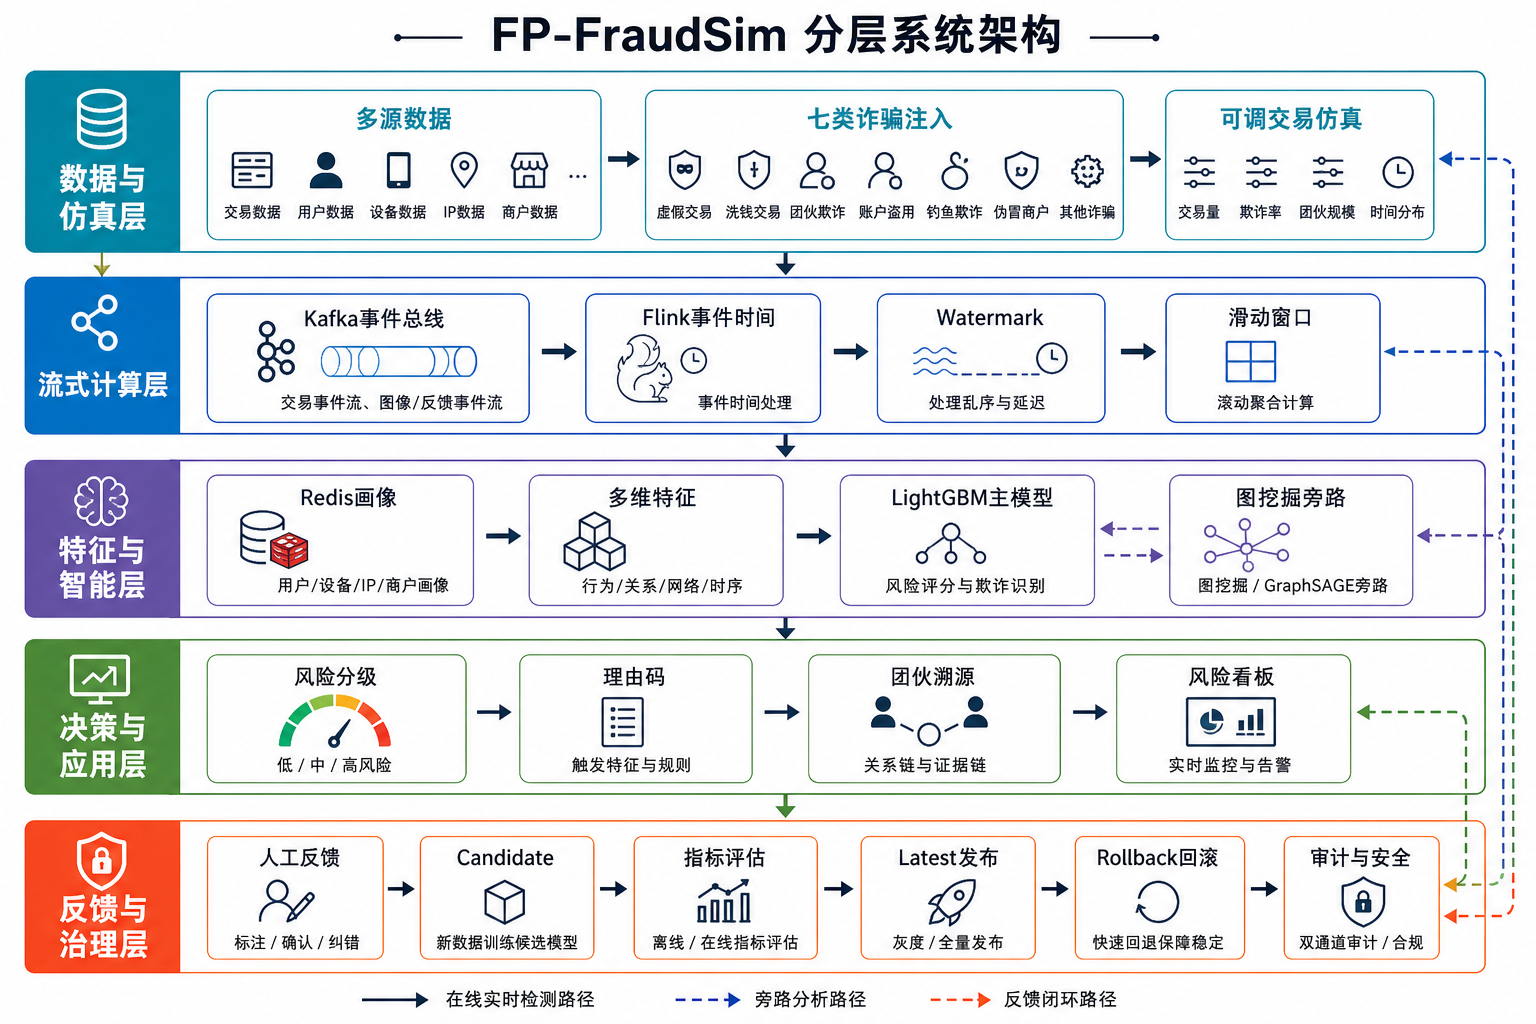
\includegraphics[width=\textwidth]{pic/layered_system_architecture_image2.png}
  \caption{FP-FraudSim分层系统架构与闭环路径}
  \label{fig:fraudsim_architecture}
\end{figure}

部署上使用Docker Compose编排Kafka、Redis、Model API、Flink JobManager、Flink TaskManager和Flink风险作业，完成单机最小闭环验证。项目进一步提供\code{deploy/k8s/edge.yaml}和\code{center.yaml}：边缘/私有云实时侧部署Kafka、Redis、双副本Model API、Flink和NetworkPolicy；中心云训练侧以CronJob运行反馈候选训练和GraphSAGE旁路实验。清单包含PVC、Secret和资源约束，为后续接入对象存储、镜像仓库和跨云加密同步提供基础。

\subsubsection{框架选型与流式框架}

系统架构围绕实时反诈业务约束进行选型，而非简单堆叠组件。Kafka承担高吞吐事件总线，将交易生产、风险计算、告警和反馈解耦；即使模型服务短时波动，交易事件仍可在消息队列中保留并重放。Flink提供有状态计算、事件时间、watermark和checkpoint机制，能够在乱序交易流中稳定维护短时行为窗口，这是普通HTTP同步调用或定时批处理难以完整实现的能力。Redis以键值方式保存用户、设备、IP、商户和图画像，使在线链路无需重复扫描历史数据即可完成毫秒级画像补齐。FastAPI将模型推理独立为服务，使模型训练、流计算和推理资源能够分别扩缩容，并通过统一接口支持模型热切换。

该组合兼顾了\textbf{吞吐、延迟、容错、扩展与迭代}：Kafka和Flink适合交易流水平扩展；checkpoint和结果主题支持故障恢复与审计；Redis降低在线特征读取成本；模型服务与流计算解耦，使算法升级不需要重写实时链路。系统同时提供同步单笔和微批评分模式，能够根据业务流量在即时响应与吞吐效率之间动态取舍。

\subsection{业务逻辑流程设计}

交易流从\code{transaction\_events}主题进入Flink。在线评分作业\code{fraudsim/streaming/flink\_job.py}实现两种评分模式：同步单笔评分和微批评分。微批模式根据批大小和等待时间聚合记录，默认批大小为50、等待时间为300毫秒，再调用FastAPI批量\code{/predict}接口，以降低HTTP调用开销。

Flink作业对每条交易执行以下步骤：

\begin{enumerate}
  \item 解析JSON事件并提取事件时间；
  \item 维护用户、设备、IP、商户四类内存滑动窗口；
  \item 计算5分钟、10分钟和1小时窗口特征；
  \item 从Redis读取用户、设备、IP、商户和图画像；
  \item 调用模型服务输出风险分数、等级、处置动作和理由码；
  \item 将完整结果写入\code{risk\_results}，将高风险结果写入\code{alert\_events}，将迟到事件写入\code{late\_events}。
\end{enumerate}

该设计满足赛题关于“交易发生的同时完成风险评估与欺诈判定”的要求，同时保留结果主题便于回放、审计和答辩展示。

图~\ref{fig:realtime_decision_flow}进一步展示了单笔交易从进入流式链路到形成业务处置的过程。模型分数不是最终结果，系统还需要结合阈值、理由码和图证据生成可执行决策。

\begin{figure}[H]
  \centering
  \resizebox{\textwidth}{!}{%
  \begin{tikzpicture}[node distance=0.62cm and 0.55cm]
    \node[flowcard=flowcyan] (event) {\textcolor{white}{\bfseries 交易事件}\nodepart{second}Kafka输入};
    \node[flowcard=flowblue, right=of event] (feature) {\textcolor{white}{\bfseries Flink实时特征}\nodepart{second}窗口统计\\画像补齐};
    \node[flowcard=flowpurple, right=of feature] (score) {\textcolor{white}{\bfseries 模型服务}\nodepart{second}风险分数\\理由码};
    \node[decisioncard, right=0.7cm of score] (decision) {两级阈值判断};
    \node[flowcard=flowgreen, above right=0.55cm and 0.8cm of decision] (pass) {\textcolor{white}{\bfseries 低风险}\nodepart{second}直接放行};
    \node[flowcard=floworange, right=0.8cm of decision] (review) {\textcolor{white}{\bfseries 中风险}\nodepart{second}人工复核};
    \node[flowcard=flowred, below right=0.55cm and 0.8cm of decision] (reject) {\textcolor{white}{\bfseries 高风险}\nodepart{second}拒绝并告警};
    \draw[flowarrow] (event) -- (feature);
    \draw[flowarrow] (feature) -- (score);
    \draw[flowarrow] (score) -- (decision);
    \draw[flowarrow] (decision) -- node[flowlabel, above, sloped]{低于审核阈值} (pass);
    \draw[flowarrow] (decision) -- node[flowlabel, above]{介于两阈值} (review);
    \draw[flowarrow] (decision) -- node[flowlabel, below, sloped]{高于拦截阈值} (reject);
  \end{tikzpicture}
  }
  \caption{实时风险评分与分级处置流程}
  \label{fig:realtime_decision_flow}
\end{figure}

\subsection{数据结构设计与组织}

系统以交易事实表为中心，通过画像表、图结构和事件主题组织数据。离线Parquet保证大规模分析与可复现训练效率，在线JSON事件保证Kafka传输兼容性，Redis键值画像保证低延迟查询，图节点与图边保证团伙关系可追溯。核心结构如表~\ref{tab:data_structure_design}所示。

\begin{table}[H]
  \centering
  \caption{核心数据结构与组织方式}
  \label{tab:data_structure_design}
  \renewcommand\arraystretch{1.32}
  \setlength{\tabcolsep}{4pt}
  {\songti\zihao{5}
  \begin{tabularx}{0.97\textwidth}{>{\raggedright\arraybackslash}p{2.4cm}>{\raggedright\arraybackslash}p{2.5cm}>{\raggedright\arraybackslash}X>{\raggedright\arraybackslash}p{3.1cm}}
    \toprule
    数据对象 & 存储/传输形式 & 核心内容 & 作用 \\
    \midrule
    交易事实表 & Parquet / JSON事件 & 交易ID、事件时间、主体、金额、渠道、设备、IP、标签 & 训练基表与实时输入 \\
    实体画像 & Parquet / Redis Hash & 用户、设备、IP、商户历史统计与风险属性 & 毫秒级在线特征补齐 \\
    短时窗口状态 & Flink Keyed State & 5分钟、10分钟、1小时计数、金额和唯一实体数 & 捕捉实时突发异常 \\
    异构关系图 & 节点表、边表、证据JSONL & 用户、交易、设备、IP、商户、收款方及关系 & 团伙识别与链路溯源 \\
    模型与指标 & Pickle / JSON / Parquet & 模型、特征配置、阈值、评估分数和排行榜 & 受控评估、发布与回滚 \\
    事件主题 & Kafka Topics & 交易、风险结果、告警、迟到、反馈和审计事件 & 解耦、回放与审计 \\
    \bottomrule
  \end{tabularx}}
\end{table}

\subsection{算法模型和伪代码}

\subsubsection{算法组合的合理性与先进性}

反诈识别同时包含“已知欺诈模式分类”“短时异常发现”和“团伙关系挖掘”三个不同问题，单一算法难以兼顾。因此，本系统采用分层组合算法：

\begin{enumerate}
  \item \textbf{梯度提升模型负责交易级综合判别。}支付风控数据以结构化数值和类别特征为主，并存在大量非线性交互。LightGBM等梯度提升模型在此类数据上具有较强效果、较低推理成本和较成熟的特征贡献分析能力，适合作为在线主模型；XGBoost、CatBoost和sklearn模型通过统一适配器作为对照与备选。
  \item \textbf{滑动窗口特征负责动态异常检测。}模型不仅观察交易当前值，还实时计算用户5分钟交易频次、设备/IP 10分钟关联用户数、商户1小时集中度等特征，使突发高频、批量账号和集中收单等行为在发生时被量化。
  \item \textbf{图挖掘与GraphSAGE旁路负责团伙结构研究。}共享资源筛选与连通分量算法将分散交易还原为可解释证据网络；两层GraphSAGE通过受控采样学习节点嵌入，用于验证图表示价值。图模型当前保持旁路，避免未经充分时序验证的嵌入影响线上LightGBM稳定性。
  \item \textbf{阈值校准、阈值沙盒与理由码负责业务决策。}系统不固定使用0.5阈值，而是将模型分数映射为拒绝、复核和放行；阈值沙盒进一步量化误报成本、欺诈召回与人工审核容量之间的权衡。
\end{enumerate}

这种“监督模型 + 实时窗口 + 图关系 + 决策解释”的组合，将先进算法能力嵌入可执行的业务链路，兼顾准确性、实时性与可解释性。

\begin{algorithm}[H]
\caption{实时诈骗判定与分级处置}
\label{alg:realtime_fraud_decision}
\KwIn{交易事件$e$，实体画像$P$，窗口状态$W$，图风险$G$，审核阈值$T_1$，拦截阈值$T_2$}
\KwOut{风险分数$s$，风险等级$l$，处置动作$a$，理由码$R$}
校验事件并按事件时间更新$W$\;
从Redis读取用户、设备、IP和商户画像，构造多维特征$x \leftarrow f(e,P,W,G)$\;
使用主模型计算$s \leftarrow \mathrm{LightGBM}(x)$，并生成理由码$R$\;
\eIf{$s \ge T_2$}{
  $l \leftarrow$高风险，$a \leftarrow$拦截并告警；写入风险结果、告警和审计主题\;
}{
  \eIf{$s \ge T_1$}{
    $l \leftarrow$中风险，$a \leftarrow$人工复核；展示理由码与证据链\;
  }{
    $l \leftarrow$低风险，$a \leftarrow$放行；保留结果用于回放\;
  }
}
将复核标签写入反馈样本池，供阈值调优和候选模型训练\;
\end{algorithm}

\subsubsection{模型训练与多模型管理}

训练入口为\code{fraudsim/training/train.py}。脚本读取训练、验证和测试切分，合并窗口特征和图特征，自动剔除ID字段、控制字段和泄露字段，随后调用模型注册表中的适配器进行训练。当前项目支持LightGBM、XGBoost、CatBoost、sklearn逻辑回归、HistGradientBoosting等模型适配器，所有模型共享统一的特征配置、指标输出和产物目录结构。

训练产物包括：

\begin{itemize}
  \item \code{model.pkl}：模型本体、模型元数据和特征配置；
  \item \code{feature\_config.json}：特征列、类别列和数值缺失填充值；
  \item \code{metrics.json}：PR-AUC、ROC-AUC、F1、Top 1\%召回、误报率和阈值校准报告；
  \item \code{leaderboard.json}：不同模型在同一数据集上的排行榜。
  \item \code{evaluation\_scores.parquet}：阈值沙盒使用的测试标签与风险分数。
\end{itemize}

人工反馈通过\code{/feedback}同时写入Kafka的\code{feedback\_events}主题和本地反馈样本池。自适应训练脚本基于反馈生成\code{candidate}候选模型；\code{/models/promote}在发布前将当前\code{latest}备份为\code{rollback}，\code{/models/rollback}可快速恢复旧版本。该candidate/latest/rollback三段式生命周期避免新反馈样本直接覆盖线上模型。

模型迭代采用受控闭环，如图~\ref{fig:model_lifecycle}所示。候选模型必须先完成离线评估与人工确认，发布失败或线上异常时可恢复回滚版本，避免自动重训直接影响实时交易。

\begin{figure}[H]
  \centering
  \resizebox{\textwidth}{!}{%
  \begin{tikzpicture}[node distance=0.7cm and 0.75cm]
    \node[flowcard=flowcyan] (feedback) {\textcolor{white}{\bfseries 人工复核}\nodepart{second}反馈标签};
    \node[flowcard=flowblue, right=of feedback] (pool) {\textcolor{white}{\bfseries 反馈样本池}\nodepart{second}质量检查\\样本合并};
    \node[flowcard=flowpurple, right=of pool] (candidate) {\textcolor{white}{\bfseries Candidate}\nodepart{second}候选模型训练};
    \node[flowcard=floworange, right=of candidate] (evaluate) {\textcolor{white}{\bfseries 离线评估}\nodepart{second}指标与冒烟测试};
    \node[flowcard=flowgreen, right=of evaluate] (latest) {\textcolor{white}{\bfseries Latest}\nodepart{second}线上活动模型};
    \node[flowcard=flowred, below=0.75cm of latest] (rollback) {\textcolor{white}{\bfseries Rollback}\nodepart{second}历史稳定版本};
    \draw[flowarrow] (feedback) -- (pool);
    \draw[flowarrow] (pool) -- (candidate);
    \draw[flowarrow] (candidate) -- (evaluate);
    \draw[flowarrow] (evaluate) -- node[flowlabel, above]{确认发布} (latest);
    \draw[flowarrow] (latest) -- node[flowlabel, right]{发布前备份} (rollback);
    \draw[flowarrow] (rollback.west) -| node[flowlabel, below, pos=0.25]{异常恢复} (evaluate.south);
    \draw[flowarrow] (latest.north) |- ++(0,0.65) -| node[flowlabel, above, pos=0.25]{新反馈继续进入闭环} (feedback.north);
  \end{tikzpicture}
  }
  \caption{反馈驱动的候选模型发布与回滚闭环}
  \label{fig:model_lifecycle}
\end{figure}

\subsubsection{风险解释与理由码}

API不仅输出风险分数，还根据交易上下文生成理由码。理由码规则位于\code{fraudsim/api/app.py}，覆盖金额偏离、高频交易、共享设备、风险IP、商户集中、欺诈邻域、团伙命中、共享IP集群等原因。例如，当交易金额超过用户平均金额三倍且超过绝对金额阈值时输出\code{amount\_deviation}；当设备10分钟内关联多个用户或历史绑定用户数过高时输出\code{shared\_device}；当付款方图挖掘团伙风险分较高时输出\code{fraud\_ring\_detected}。

理由码的作用是把黑盒模型输出转化为可解释证据，辅助人工复核和策略调优。对于高风险但未触发具体规则的交易，系统补充\code{model\_high\_score}，提示该风险主要来自模型综合判别。

图~\ref{fig:operation_scenarios}展示了欺诈行为产生的异常线索，图~\ref{fig:fraud_judgment_illustration}进一步说明系统如何完成诈骗判定：交易进入实时链路后，金额偏离、短时高频、设备/IP共享、风险商户和团伙关系等证据共同进入模型；模型输出连续风险分数和理由码，再由两级阈值分流为低风险放行、中风险复核和高风险拒绝告警。复核标签与处置结果回流至样本池，用于后续阈值调优和候选模型迭代。

\begin{figure}[H]
  \centering
  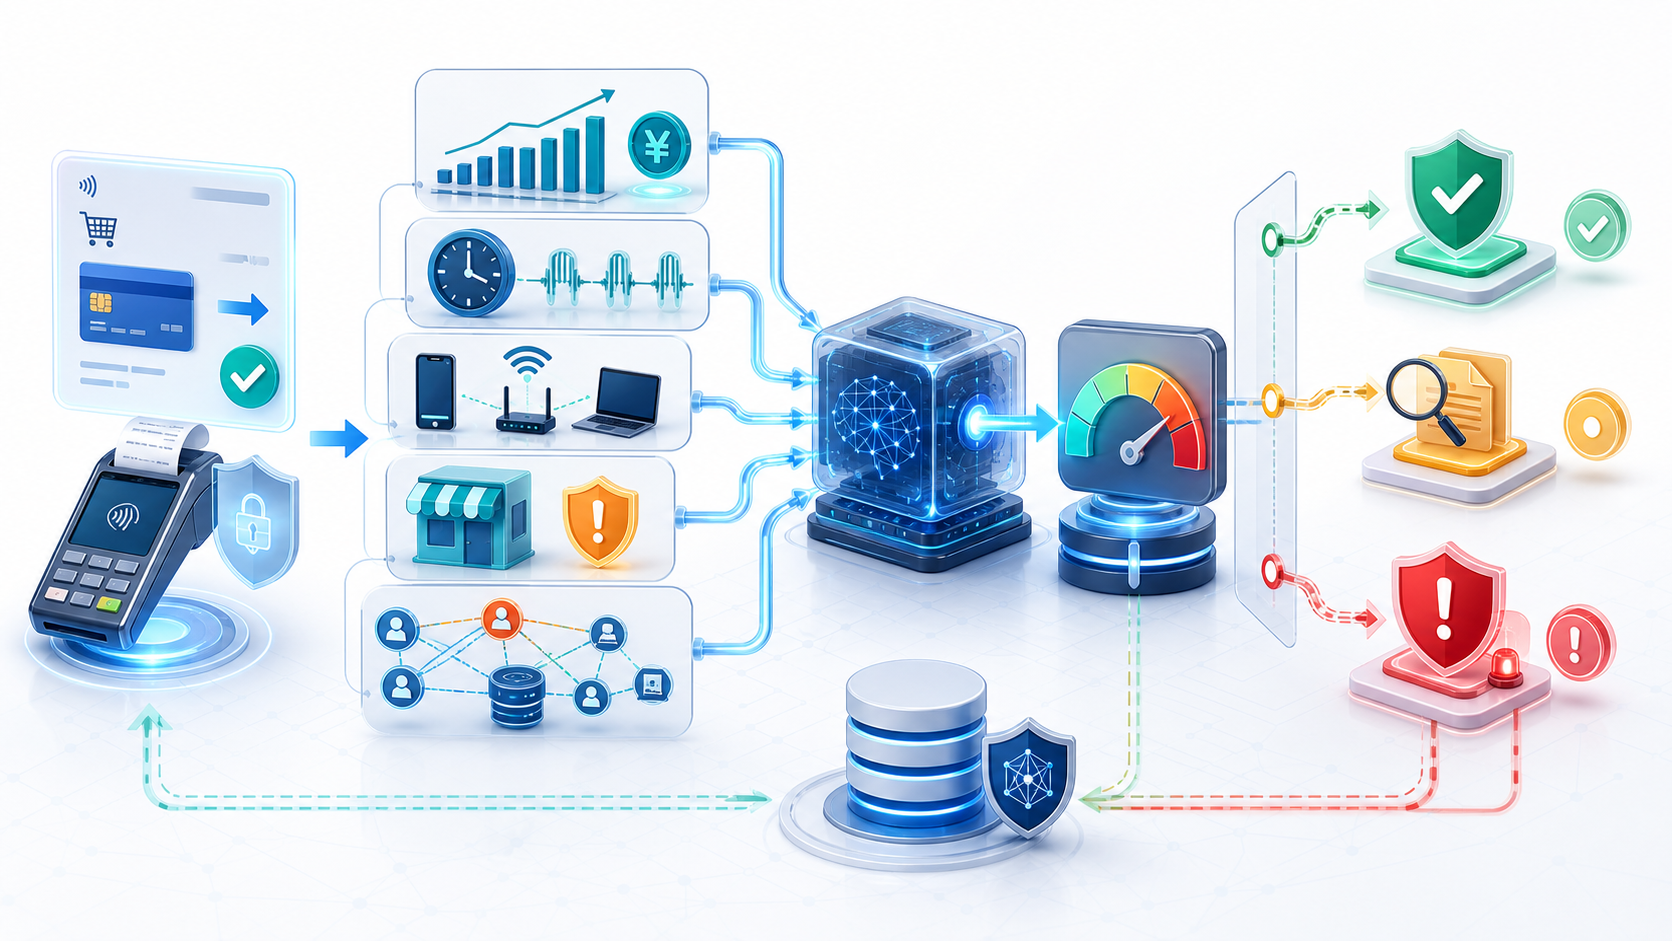
\includegraphics[width=0.92\textwidth]{pic/fraud_analyst_review.png}
  \caption{多维证据融合与诈骗分级判定示意}
  \label{fig:fraud_judgment_illustration}
\end{figure}

Dashboard将风险分数、处置结论、图链路和理由码组织在同一研判界面中，如图~\ref{fig:dashboard_reason_codes}所示。评审人员能够从高风险结论继续下钻到短时高频、共享设备、商户集中和欺诈邻域等具体证据，验证判定结果并非只有黑盒分数。

\begin{figure}[H]
  \centering
  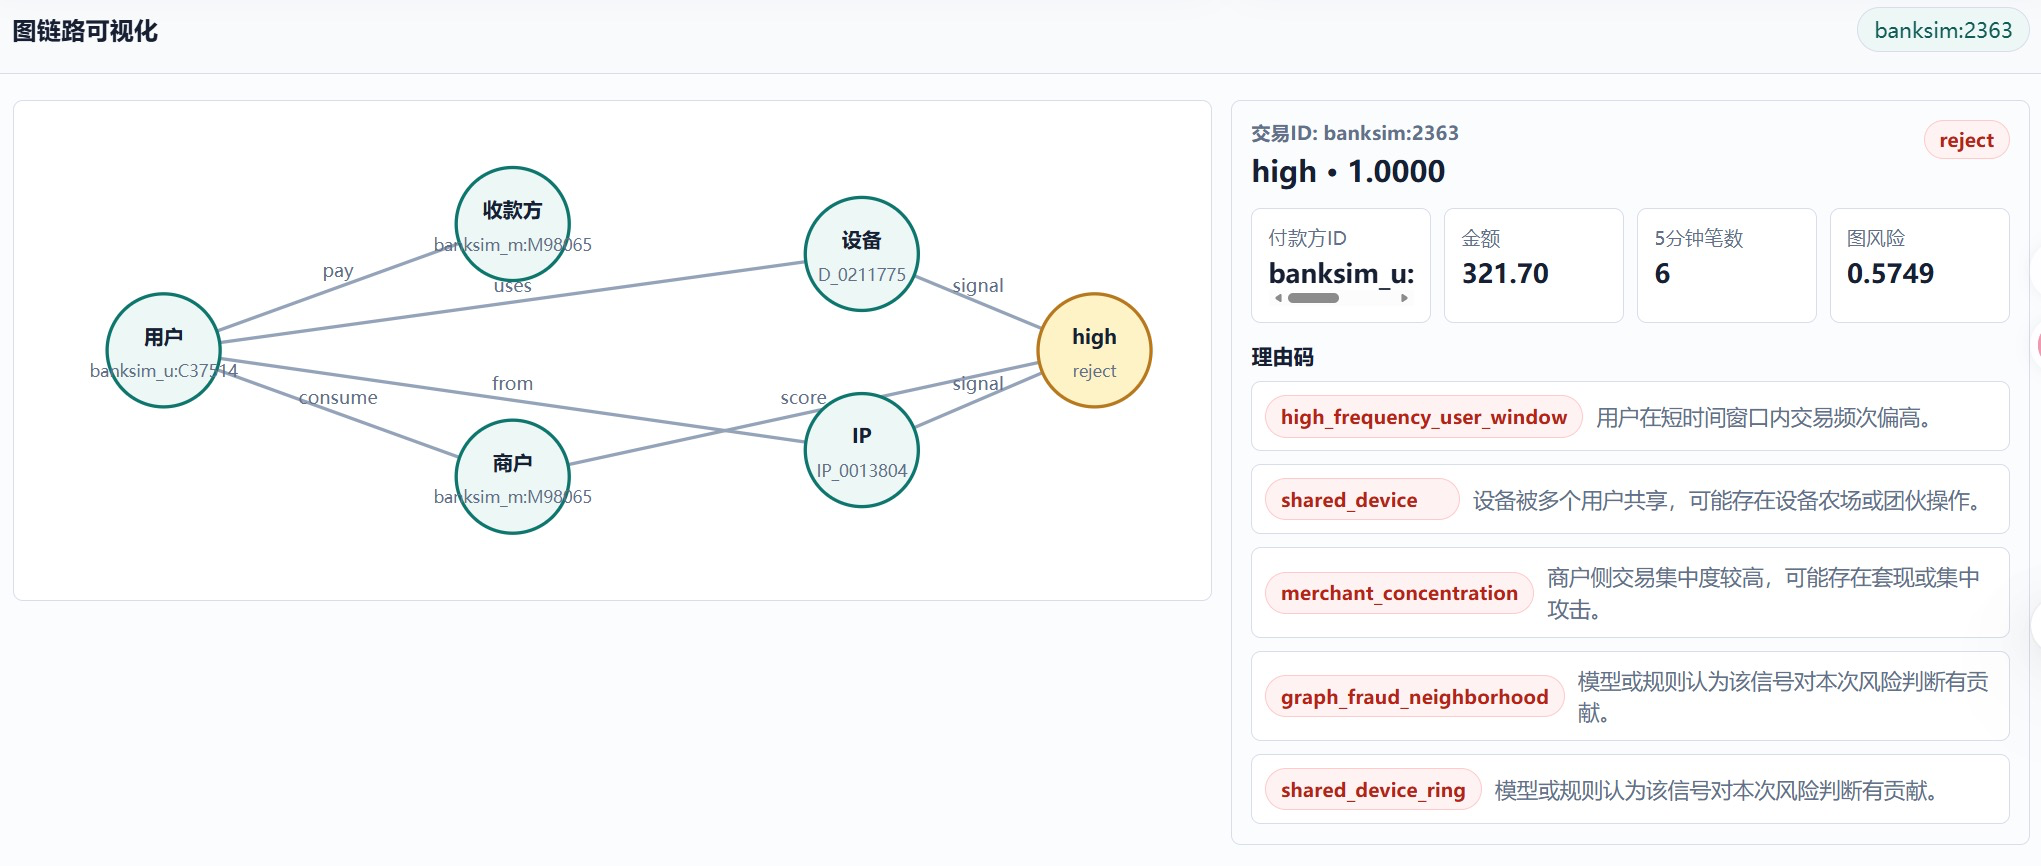
\includegraphics[width=0.96\textwidth]{pic/dashboard_reason_codes_report.png}
  \caption{单笔高风险交易的图链路与理由码解释界面}
  \label{fig:dashboard_reason_codes}
\end{figure}

\subsubsection{诈骗行为建模、图挖掘与团伙溯源}

图挖掘模块以交易、账户、设备、IP、商户和收款方为节点，以交易、登录、设备使用、商户支付、转账等关系为边。模块通过共享资源筛选候选风险资源，再使用并查集构建连通分量，综合欺诈种子比例、用户规模、证据数量、共享设备/IP数量和场景数量计算团伙风险分。

图挖掘输出四类产物：\code{fraud\_groups.parquet}记录疑似团伙列表；\code{entity\_graph\_risk.parquet}记录实体级团伙风险特征；\code{group\_evidence.jsonl}记录共享设备、IP、商户、收款方等证据；\code{graph\_mining\_summary.json}记录挖掘摘要。API提供团伙列表、团伙详情、实体风险和实体关联链路接口，Dashboard支持拖拽和缩放证据图，满足赛题对“可解释性与溯源分析”的要求。

\begin{figure}[H]
  \centering
  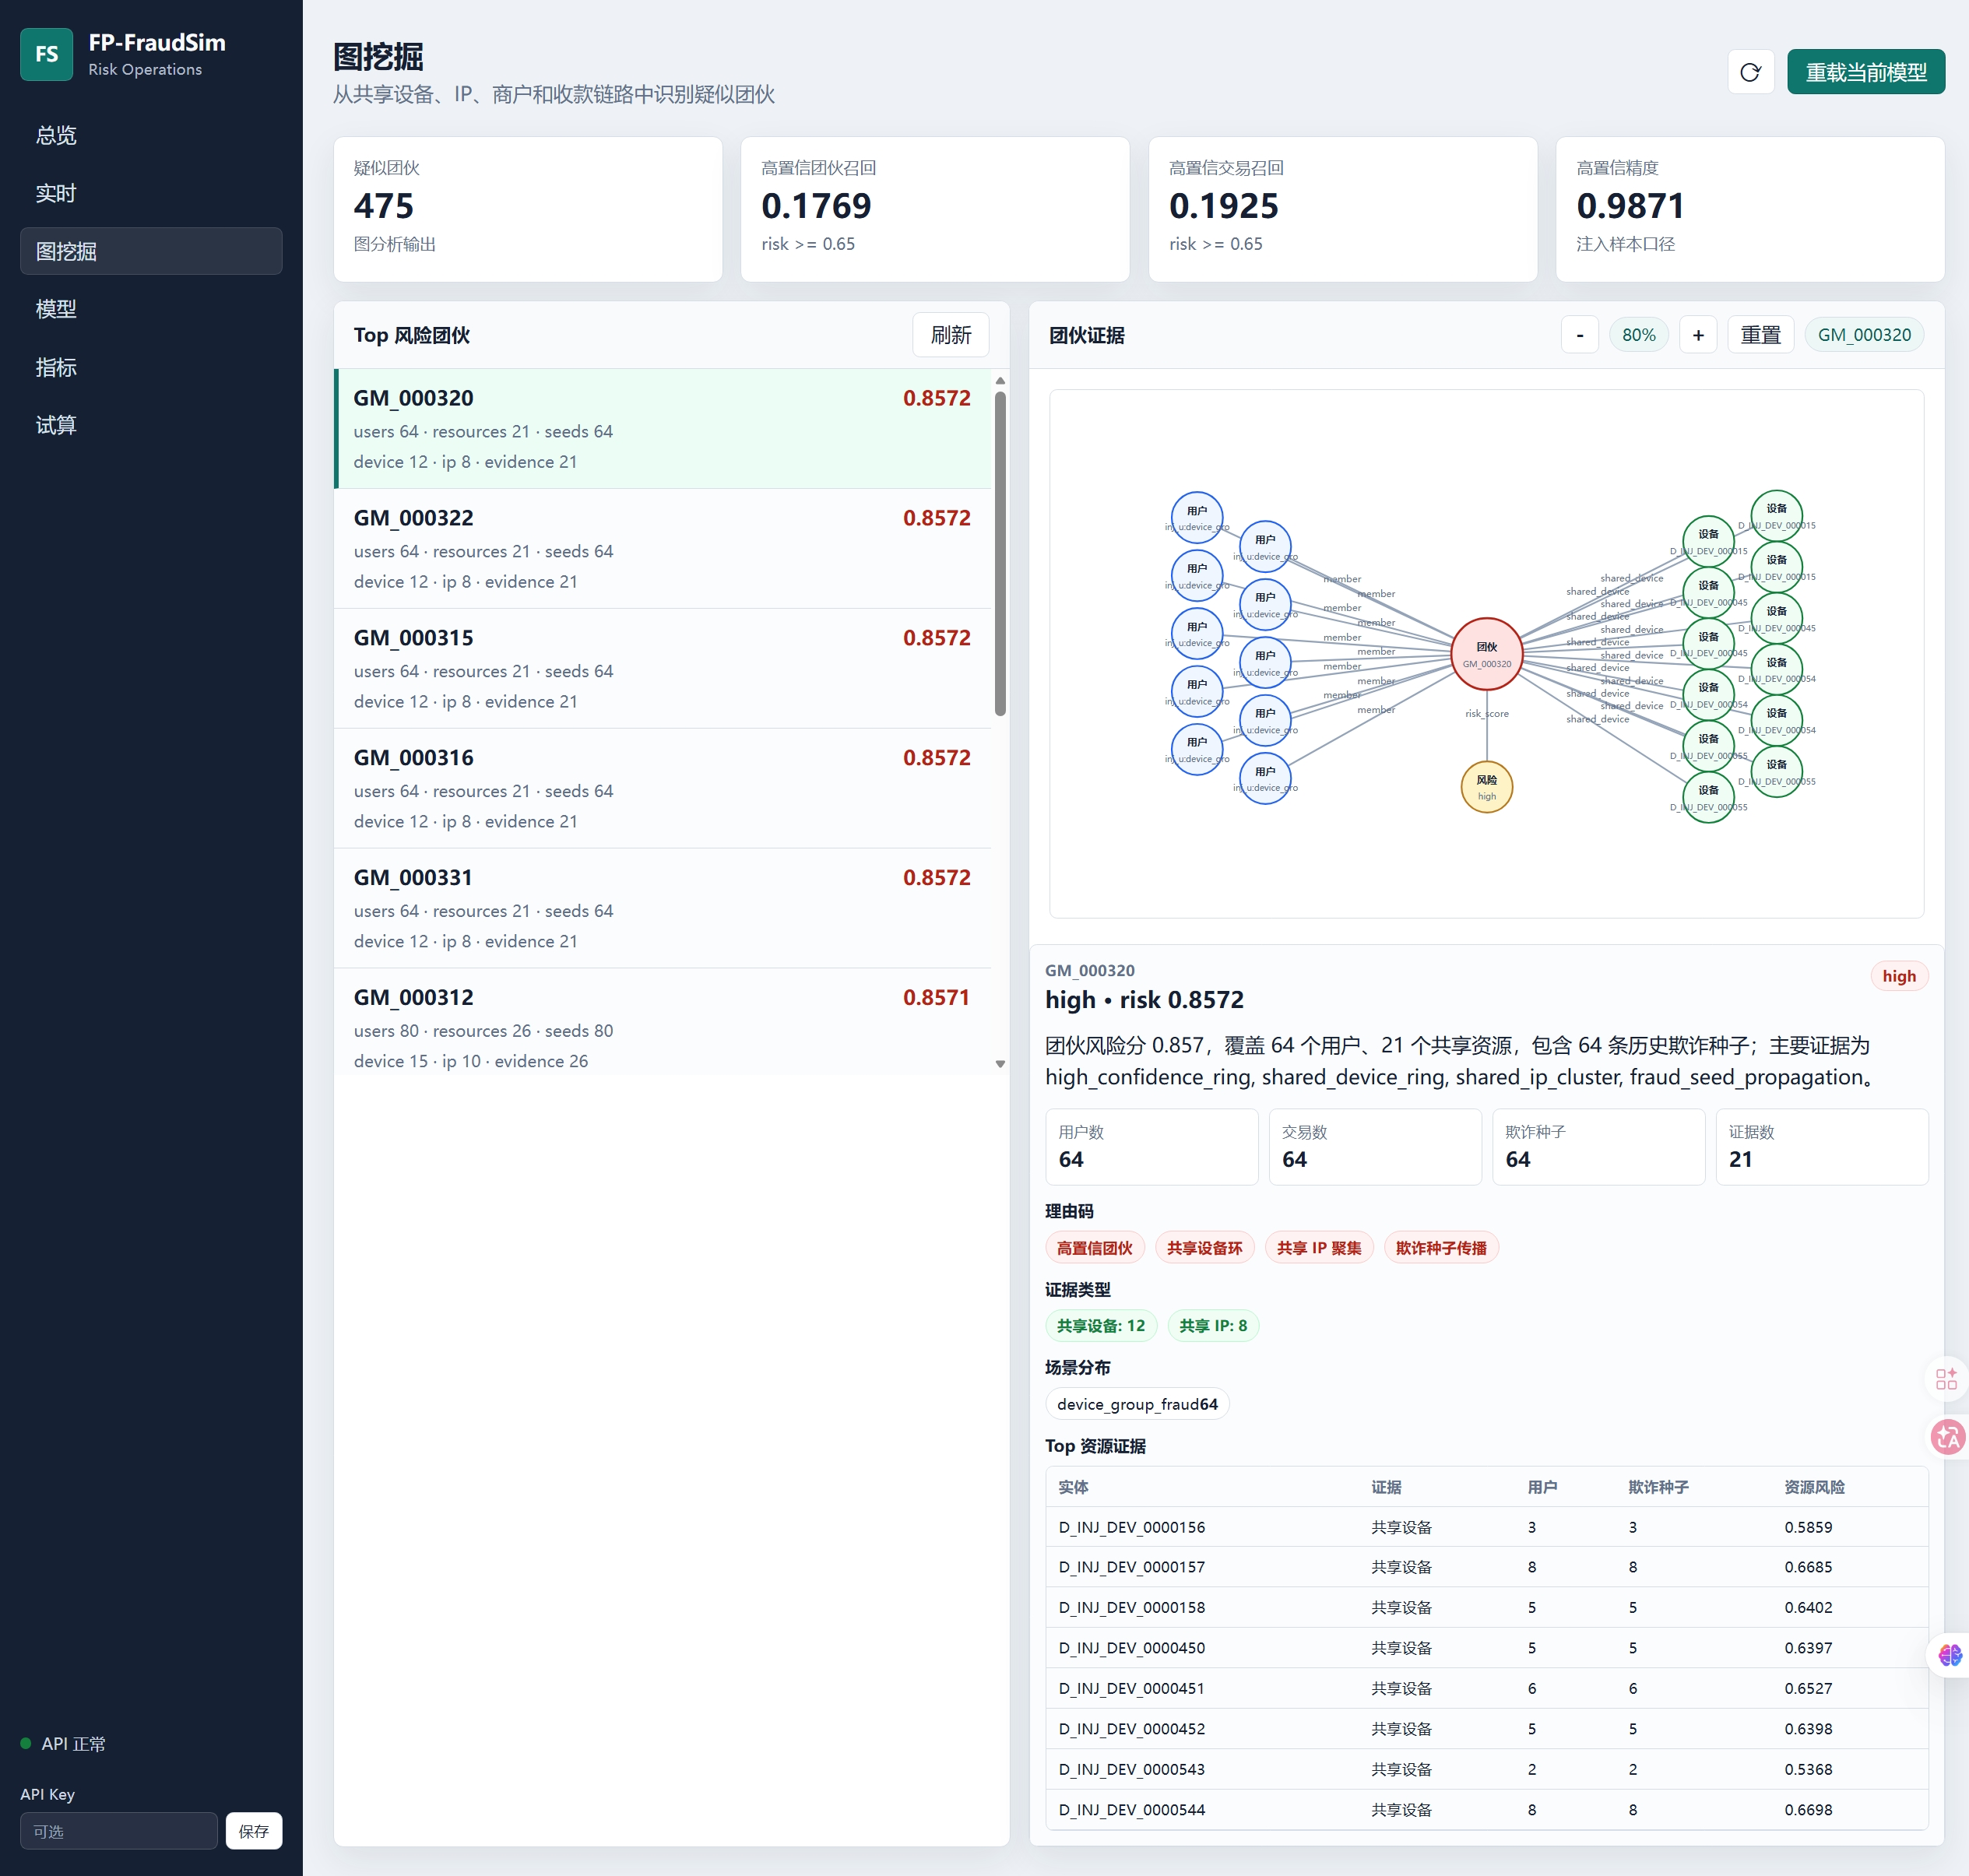
\includegraphics[width=0.76\textwidth]{pic/dashboard_fraud_groups_report.png}
  \caption{疑似欺诈团伙列表、共享资源证据与关系网络界面}
  \label{fig:dashboard_fraud_groups}
\end{figure}

GraphSAGE旁路模块从统一图边中受控采样，使用节点类型、度数和邻居聚合训练两层模型，输出模型、节点嵌入、风险分数和实验指标。线上主模型继续使用稳定的基础图统计，GraphSAGE结果用于创新验证和后续融合研究。

\subsubsection{可视化应用扩展}

Dashboard由Model API静态托管，路径为\code{/dashboard}。页面支持查看健康状态、模型指标、Kafka近期消息、实时告警、单笔试算、人工反馈、模型切换、图挖掘结果、GraphSAGE旁路指标和阈值沙盒。演示按钮封装可调仿真、画像初始化、交易回放、候选重训和图挖掘任务，API返回任务状态与日志尾部，便于在一个界面完成闭环演示。

图~\ref{fig:dashboard_overview}展示了系统总览与核心任务入口，图~\ref{fig:dashboard_replay_feedback}展示了交易回放、实时风险结果、图链路和人工反馈的联动过程。两类界面共同证明系统能够从模型加载状态进入实时识别，并将复核结论重新写回反馈主题。

\begin{figure}[H]
  \centering
  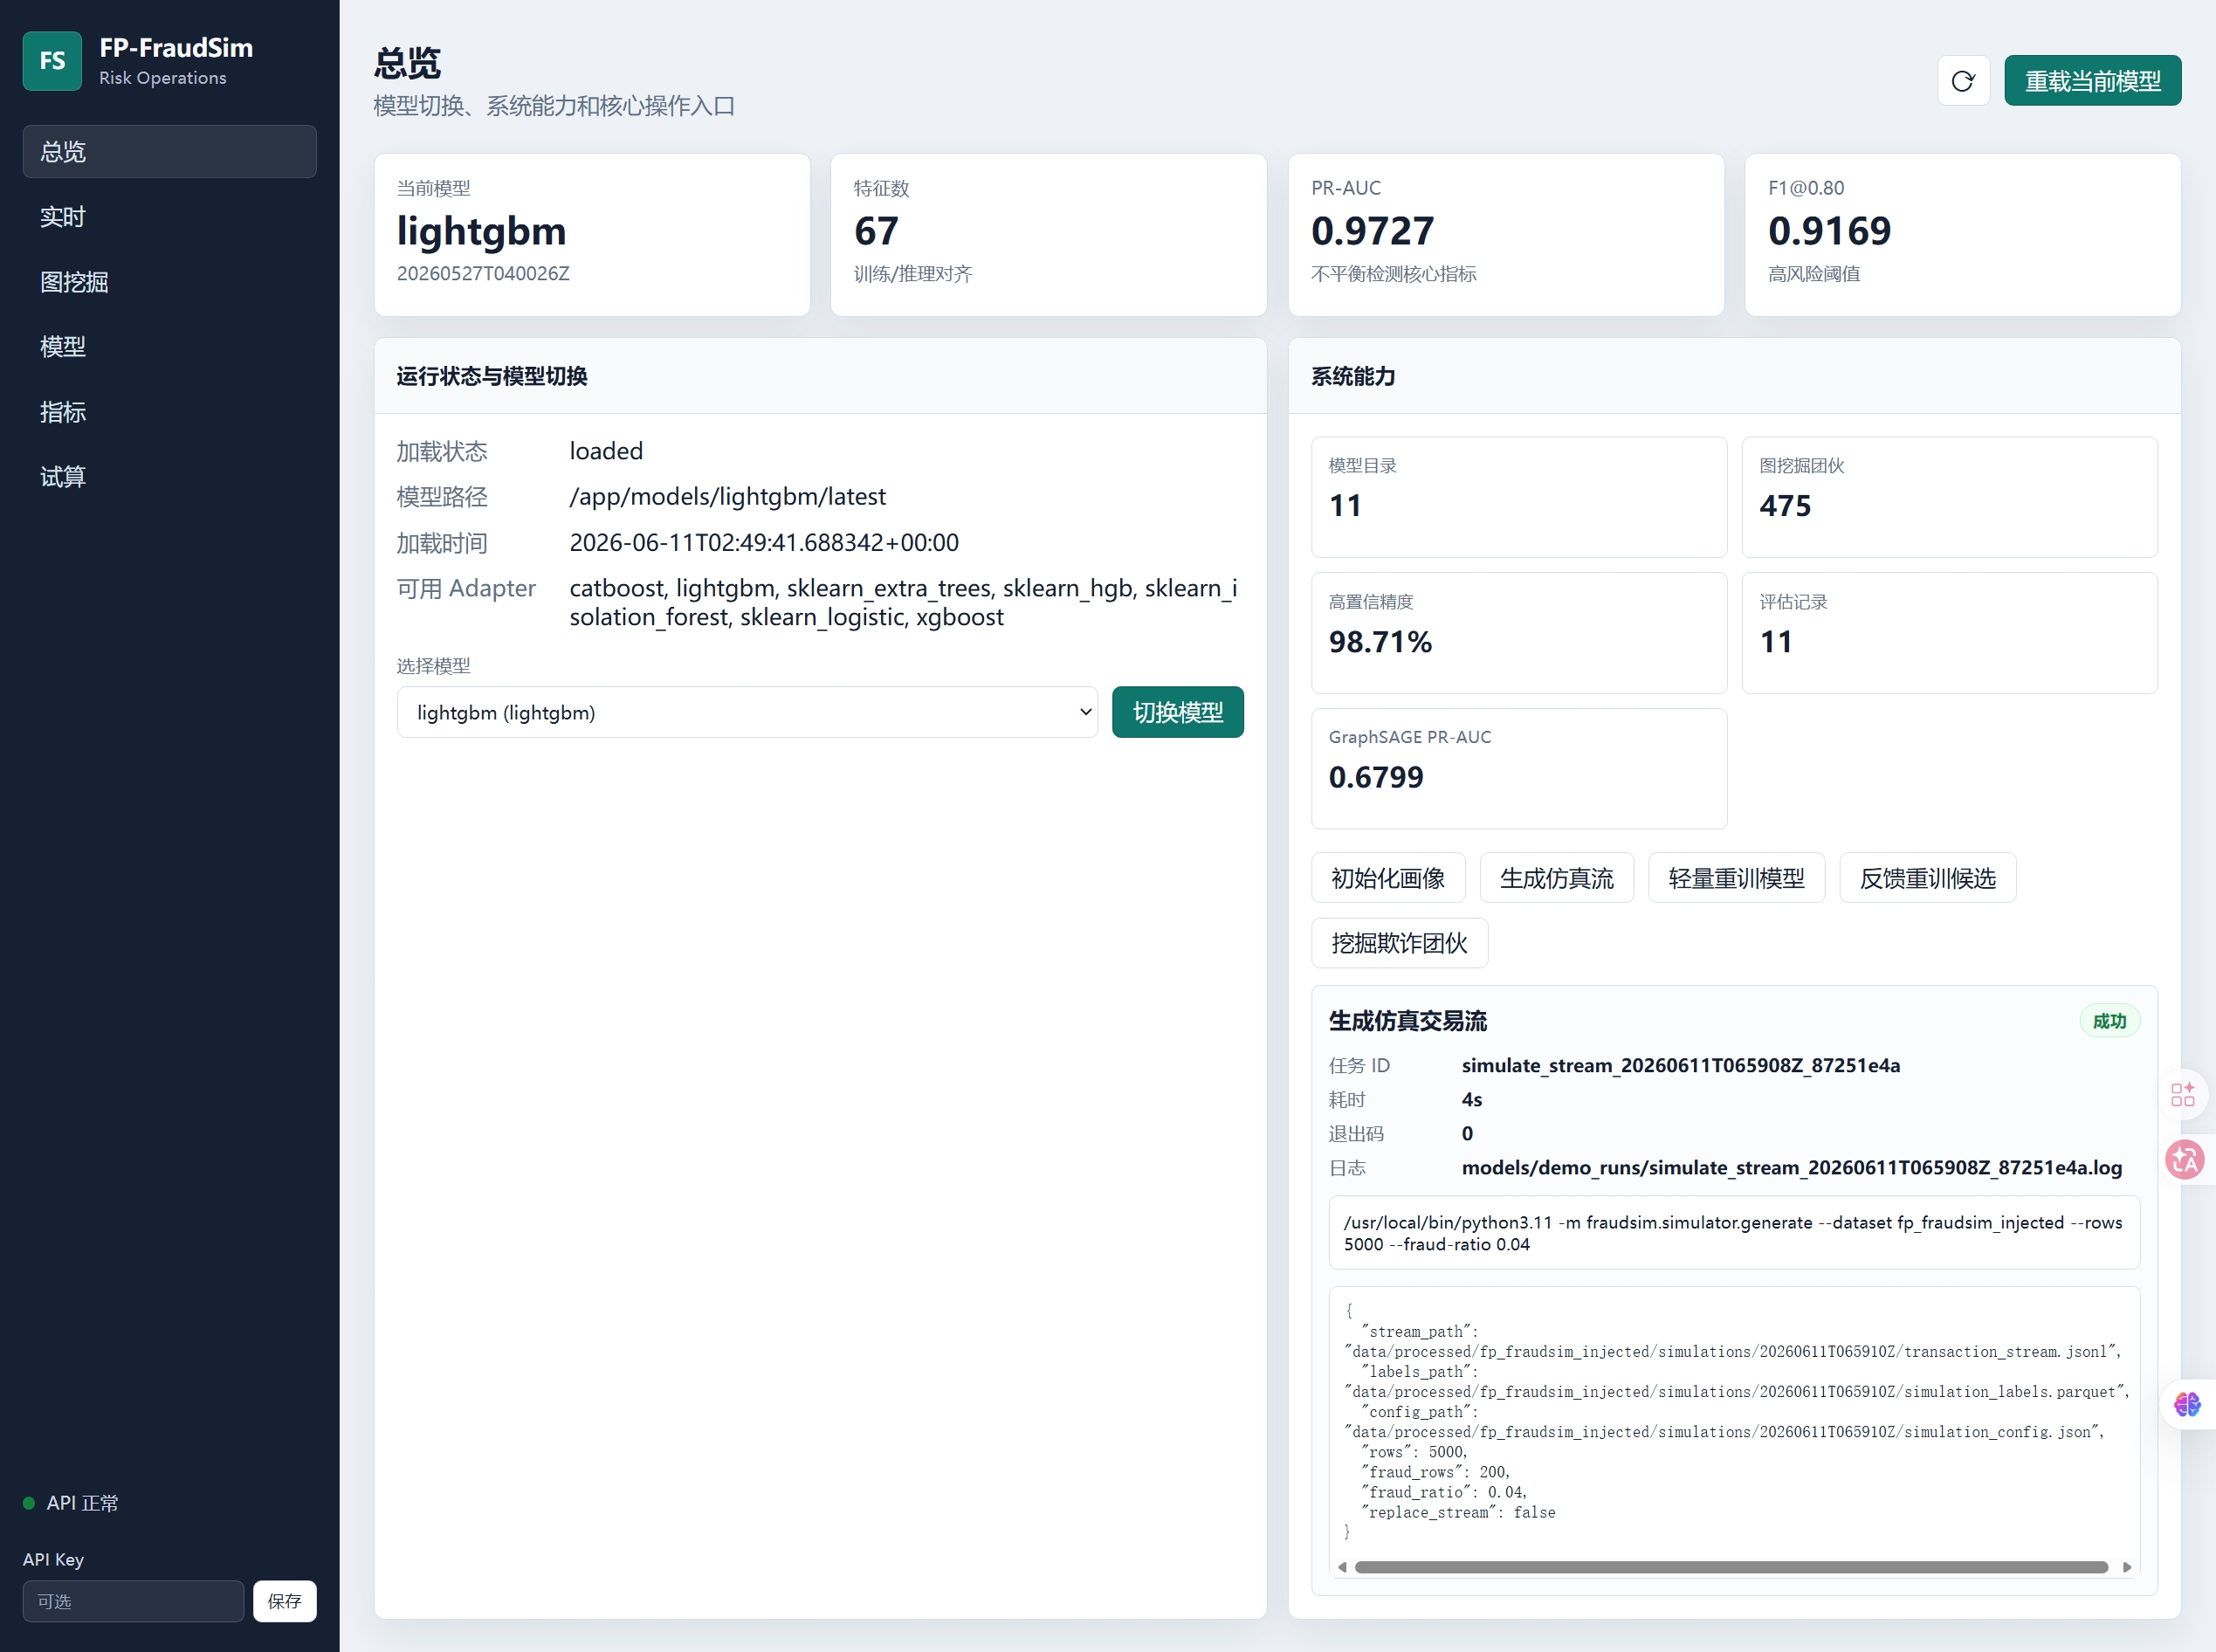
\includegraphics[width=0.90\textwidth]{pic/dashboard_overview_report.png}
  \caption{FP-FraudSim Dashboard总览与核心任务入口}
  \label{fig:dashboard_overview}
\end{figure}

\begin{figure}[H]
  \centering
  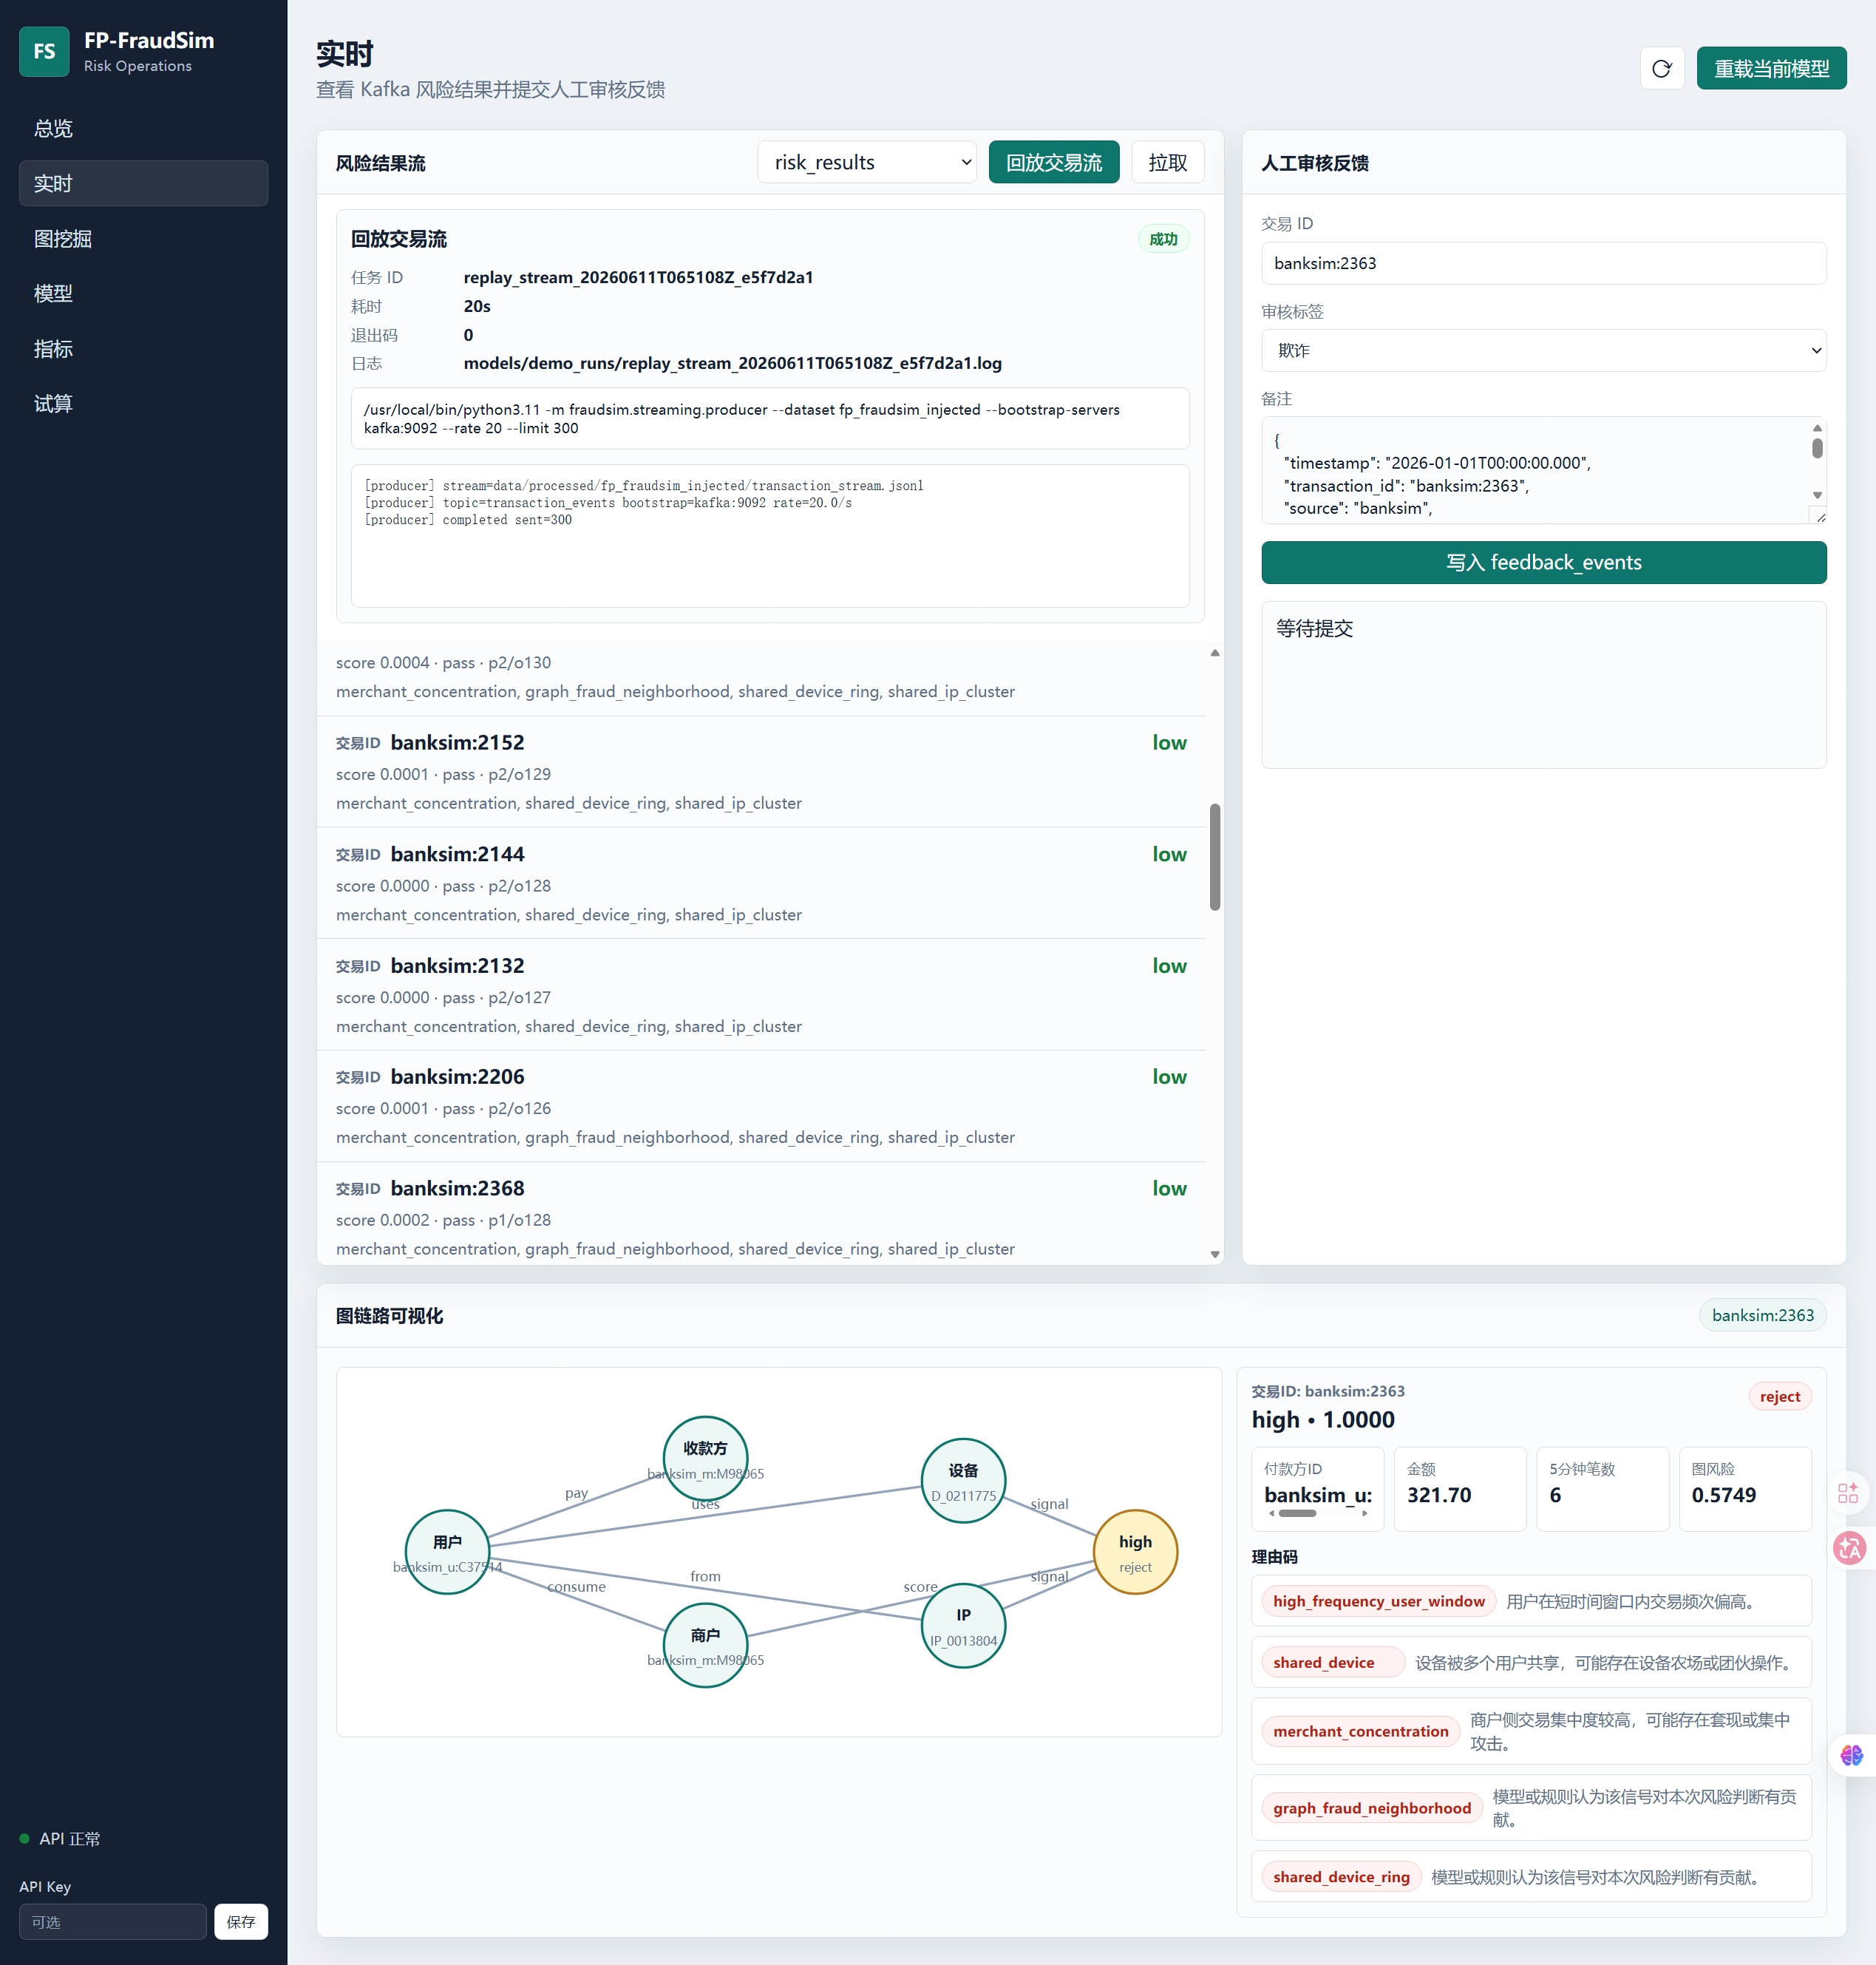
\includegraphics[width=0.74\textwidth]{pic/dashboard_replay_feedback_report.png}
  \caption{交易流回放、实时判定与人工反馈联动界面}
  \label{fig:dashboard_replay_feedback}
\end{figure}

\section{性能分析及系统展示}
\label{sec:experiment}

\subsection{围绕目标的端到端性能分析}

本作品的性能验证围绕赛题一评分要求和真实风控目标展开，重点证明系统同时具备实时性、准确性、可解释性和溯源性，而不是只报告单一分类指标。实验覆盖离线主模型、实时链路、API延迟、阈值策略、团伙挖掘、GraphSAGE旁路以及部署清单结构验证。

\begin{table}[H]
  \centering
  \caption{实验验证项目}
  \label{tab:experiment_items}
  \renewcommand\arraystretch{1.35}
  \setlength{\tabcolsep}{5pt}
  {\songti\zihao{5}
  \begin{tabularx}{0.96\textwidth}{>{\raggedright\arraybackslash}p{2.2cm}>{\raggedright\arraybackslash}X>{\raggedright\arraybackslash}X}
    \toprule
    实验类别 & 验证目标 & 对应脚本或接口 \\
    \midrule
    离线训练评估 & 比较模型PR-AUC、ROC-AUC、F1、Top 1\%召回和误报率 & \code{python -m fraudsim.training.train} \\
    实时链路验证 & 验证Kafka输入、Flink评分、告警输出和迟到事件输出 & \code{producer}、\code{flink\_job.py}、\code{/topics/\{topic\}/recent} \\
    API延迟压测 & 比较单笔评分与批量评分的平均、P50、P95、P99延迟 & \code{scripts/benchmark\_api\_latency.py} \\
    图挖掘验证 & 验证疑似团伙、共享资源证据、实体风险特征是否生成 & \code{python -m fraudsim.graph\_mining} \\
    阈值与图学习 & 验证业务阈值影响和GraphSAGE图嵌入价值 & \code{/threshold-sandbox}、\code{graphsage\_experiment} \\
    部署与安全 & 验证K8s资源结构、敏感接口认证和审计链路 & K8s单元测试、\code{/audit/recent} \\
    \bottomrule
  \end{tabularx}
  }
\end{table}

\subsubsection{准确性：离线模型与业务阈值}

训练脚本使用训练集拟合模型、验证集校准阈值、测试集报告最终指标。输出指标包括PR-AUC、ROC-AUC、F1、Top 1\%召回率和高风险阈值下误报率。其中PR-AUC适合衡量欺诈样本稀少情况下的排序质量；Top 1\%召回率模拟风控团队有限审核资源下的重点拦截能力；误报率反映正常用户体验损失。

推荐复现实验命令如下：

\begin{lstlisting}[language=bash]
python -m fraudsim.training.train --dataset fp_fraudsim_injected --model lightgbm
python -m fraudsim.training.train --dataset fp_fraudsim_injected --model xgboost
python -m fraudsim.training.train --dataset fp_fraudsim_injected --model catboost
python -m fraudsim.training.train --dataset fp_fraudsim_injected --model sklearn_hgb
\end{lstlisting}

已记录的LightGBM主模型实验使用67个特征，在123,649条测试交易上取得PR-AUC 0.9727、ROC-AUC 0.9949、F1 0.9169，高风险阈值下误报率为0.338\%。模型训练后，\code{models/leaderboard.json}按PR-AUC排序。当前代码仓库未包含大体积数据和模型产物，复现时需按README完成数据准备与训练，并以重新生成的\code{metrics.json}核验结果。

\begin{figure}[H]
  \centering
  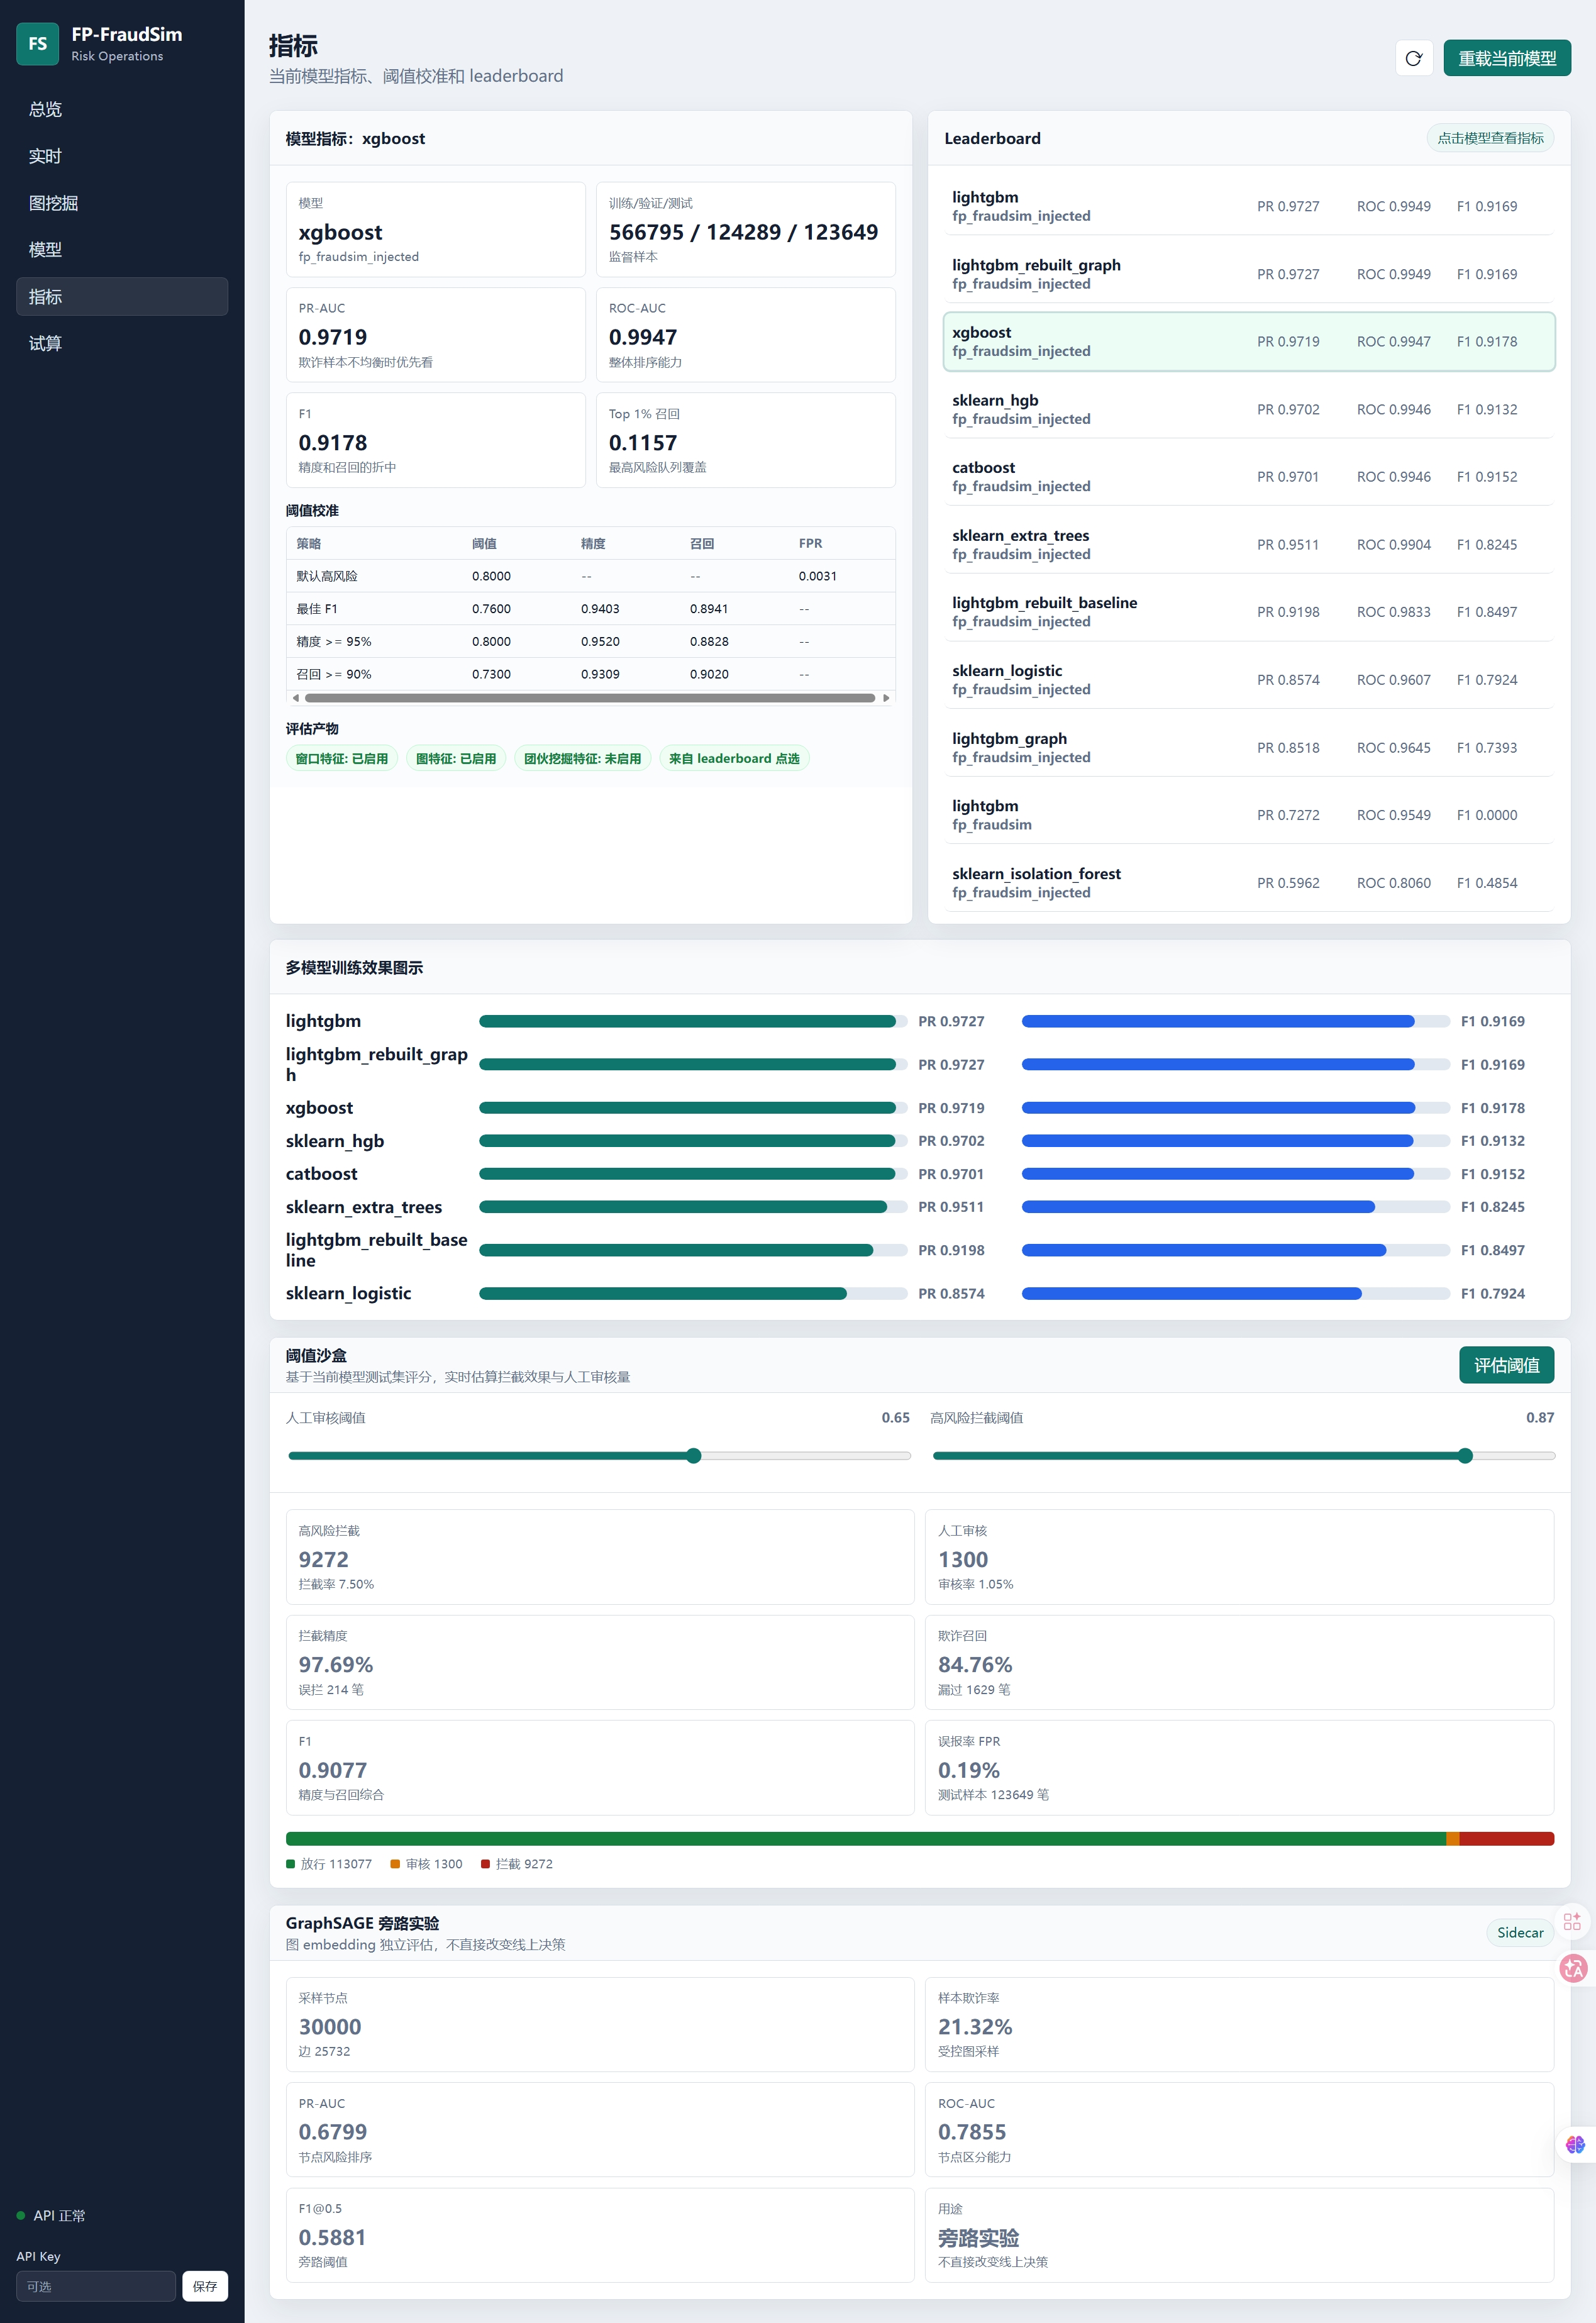
\includegraphics[width=0.68\textwidth]{pic/dashboard_model_metrics_report.png}
  \caption{多模型指标对比、排行榜与阈值评估界面}
  \label{fig:dashboard_model_metrics}
\end{figure}

\subsubsection{实时性：端到端链路与接口延迟}

系统提供Docker Compose一键部署。推荐流程为先训练模型，再启动Kafka、Redis、Model API和Flink风险作业，随后创建主题、加载画像并回放交易流。

\begin{lstlisting}[language=bash]
docker compose -p fraudsim up -d --build kafka redis model-api flink-jobmanager flink-taskmanager flink-risk-job
python -m fraudsim.streaming.topics --bootstrap-servers localhost:9094
python -m fraudsim.streaming.load_profiles --dataset fp_fraudsim_injected --redis-url redis://localhost:6379/0
python -m fraudsim.streaming.producer --dataset fp_fraudsim_injected --bootstrap-servers localhost:9094 --rate 100 --limit 1000
\end{lstlisting}

风险结果可通过Dashboard查看，也可通过API读取Kafka近期消息。实时输出字段包括\code{transaction\_id}、\code{risk\_score}、\code{risk\_level}、\code{decision}、\code{reason\_codes}、模型名称、模型版本和评分时间。该输出满足赛题要求的“风险评估、欺诈判定和风险等级输出”。

\subsubsection{接口压测与微批吞吐优化}

API延迟压测脚本先调用\code{/health}确认模型已加载，再分别测试单笔和批量\code{/predict}。本机Docker Compose实测中，单笔请求平均延迟115.78毫秒，P95为156.55毫秒，P99为240.30毫秒；每批25条时，批量请求平均耗时125.00毫秒，平均单条折算为5.00毫秒，P95折算为6.16毫秒，平均单条吞吐收益为23.16倍。

\begin{lstlisting}[language=bash]
python scripts/benchmark_api_latency.py --api-url http://localhost:8000 --records 200 --batch-size 50
\end{lstlisting}

在线流式作业默认批大小50、最长等待300毫秒，并使用flush marker主动刷新尾批。完整链路已验证Flink作业处于RUNNING状态、100条交易成功回放，\code{risk\_results}能够输出窗口、画像、图风险、决策和理由码。

\subsubsection{可解释性与溯源性：阈值和图分析}

阈值沙盒在\code{medium=0.50}、\code{high=0.80}时记录到放行112,249条、人工审核1,647条、高风险拦截9,753条，拦截精度96.08\%、欺诈召回87.69\%、误报率0.338\%。该实验说明阈值应结合误报成本和审核容量配置，而不能只以模型F1最大化为目标。

\begin{figure}[H]
  \centering
  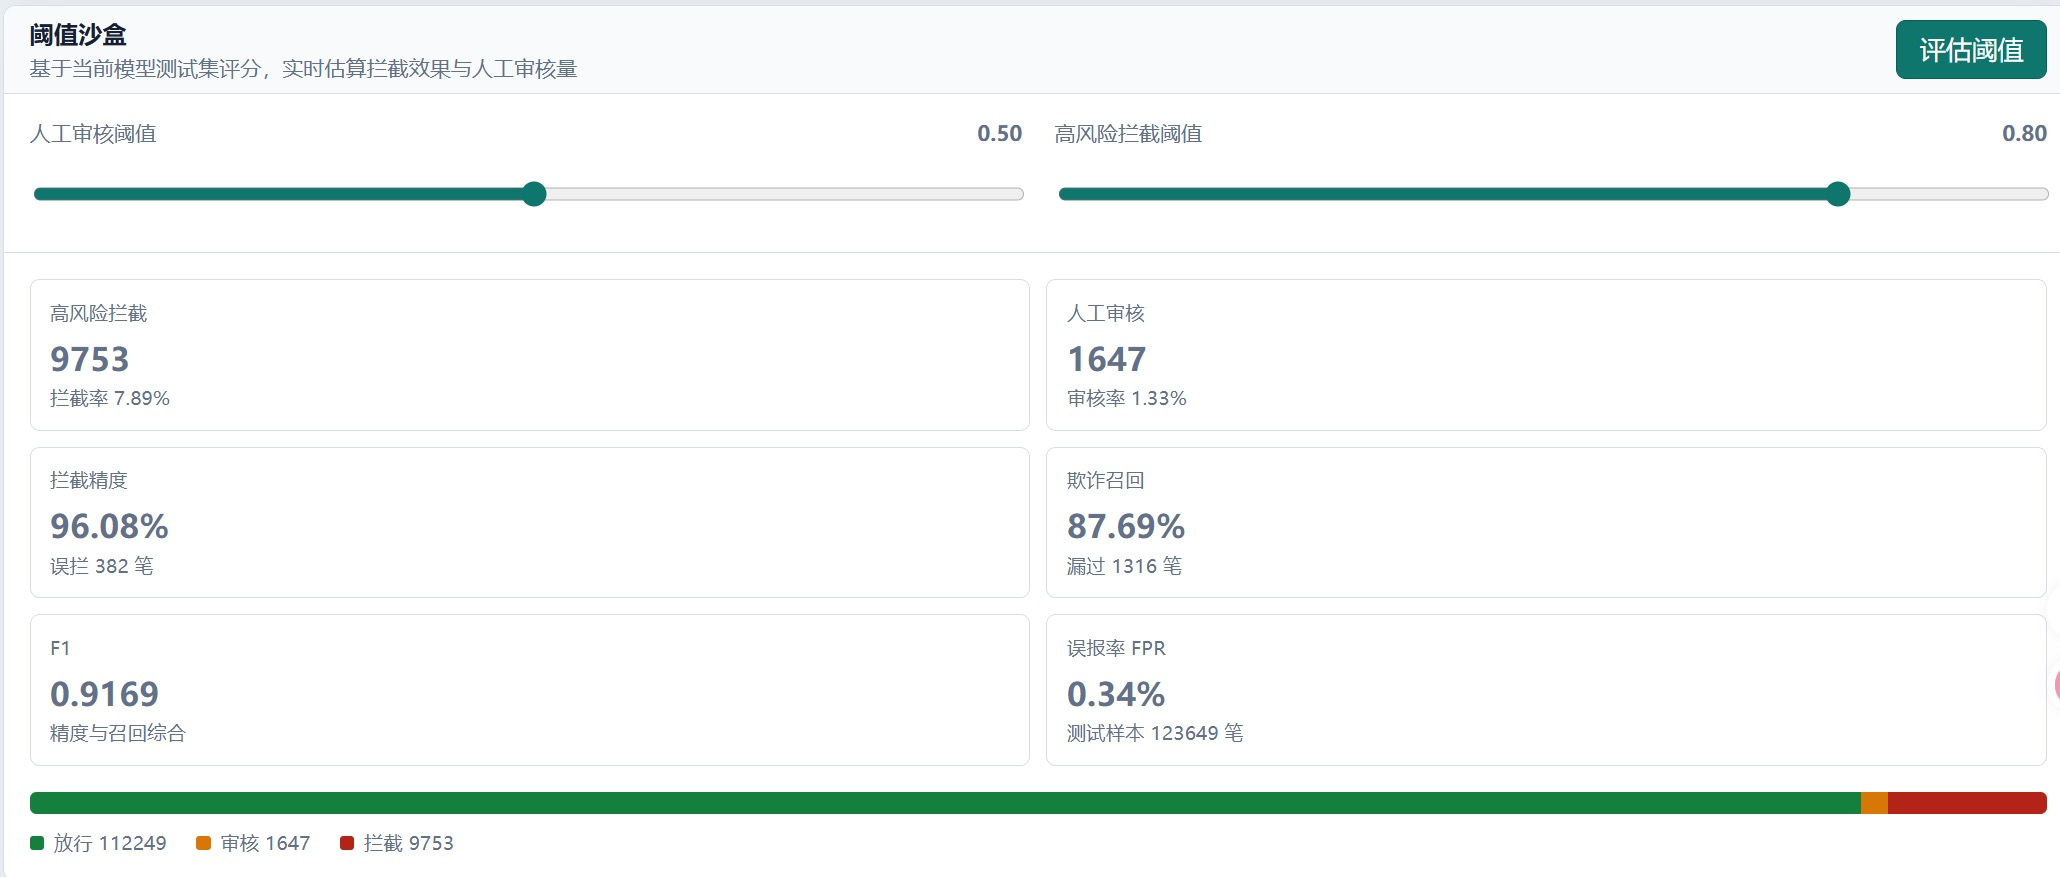
\includegraphics[width=0.96\textwidth]{pic/dashboard_threshold_report.png}
  \caption{阈值沙盒中的拦截效果与人工审核量评估}
  \label{fig:dashboard_threshold}
\end{figure}

可解释图挖掘记录到475个候选团伙；在0.65高置信阈值下，交易精度为98.71\%，注入团伙总体召回为77.93\%。GraphSAGE旁路实验采样30,000个节点和25,732条边，取得PR-AUC 0.6799、ROC-AUC 0.7855和F1@0.5为0.5881。结果证明图嵌入具有识别价值，但当前效果和时序验证尚不足以替代线上主模型，因此保持旁路。

\subsection{消融实验分析}

消融实验用于回答不同算法、参数和模块是否真正改善系统目标。表~\ref{tab:ablation_analysis}汇总当前已完成的受控对比。结果表明：微批评分显著降低单条折算耗时；图挖掘能够补充交易级模型无法直接给出的团伙证据；GraphSAGE具备研究价值，但当前指标不足以替代主模型；双阈值策略能够将模型分数转化为可控的审核工作量。

\begin{table}[H]
  \centering
  \caption{关键算法、参数与模块消融分析}
  \label{tab:ablation_analysis}
  \renewcommand\arraystretch{1.32}
  \setlength{\tabcolsep}{4pt}
  {\songti\zihao{5}
  \begin{tabularx}{0.98\textwidth}{>{\raggedright\arraybackslash}p{2.4cm}>{\raggedright\arraybackslash}p{3.0cm}>{\raggedright\arraybackslash}X>{\raggedright\arraybackslash}p{3.0cm}}
    \toprule
    对比项 & 基线/消融设置 & 关键结果 & 结论 \\
    \midrule
    单笔与微批推理 & 单笔请求；25条/批 & 单笔平均115.78ms；微批单条折算5.00ms，收益23.16倍 & 微批是高并发实时链路的关键优化 \\
    交易模型与图旁路 & LightGBM主模型；GraphSAGE旁路 & 主模型PR-AUC 0.9727；图旁路PR-AUC 0.6799 & 图嵌入暂不替代稳定主模型 \\
    无图解释与图挖掘 & 仅风险分数；增加共享资源与连通分量 & 发现475个候选团伙，高置信交易精度98.71\% & 图模块显著增强解释与溯源能力 \\
    单阈值与双阈值 & 直接二分类；$T_1=0.50,T_2=0.80$ & 形成放行112,249、复核1,647、拦截9,753的可控分流 & 双阈值连接准确率与审核容量 \\
    固定输入与可调仿真 & 固定增强集；调整欺诈率、团伙规模和速率 & 可生成不同难度和负载的复现实验流 & 增强稳定性与压力测试覆盖 \\
    \bottomrule
  \end{tabularx}}
\end{table}

\subsection{系统界面截图与任务自评}

表~\ref{tab:task_self_assessment}按照赛题一必须完成的任务进行形式检查和自评估，并给出可直接核验的界面或工程证据。自评结果用于定位交付完整性，不替代评委最终评分。

\begin{table}[H]
  \centering
  \caption{赛题一任务形式检查与自评估}
  \label{tab:task_self_assessment}
  \renewcommand\arraystretch{1.28}
  \setlength{\tabcolsep}{3.5pt}
  {\songti\zihao{5}
  \begin{tabularx}{0.98\textwidth}{>{\raggedright\arraybackslash}p{2.5cm}>{\centering\arraybackslash}p{1.2cm}>{\raggedright\arraybackslash}X>{\raggedright\arraybackslash}p{3.2cm}}
    \toprule
    必须任务 & 状态 & 核验内容 & 对应证据 \\
    \midrule
    仿真环境与实时检测 & 已完成 & 七类场景、可调仿真、交易回放与实时风险分级 & 仿真脚本、总览、回放与告警界面 \\
    流式数据处理框架 & 已完成 & Kafka、Flink事件时间、watermark、窗口与迟到分流 & Compose、Flink作业、风险主题 \\
    自适应学习与迭代 & 已完成 & 反馈样本池、Candidate、Latest、Rollback与热切换 & 回放反馈页、模型指标页、接口 \\
    多维度特征构建 & 已完成 & 交易、画像、窗口、设备/IP、商户和图关联特征 & 特征表、理由码页、图团伙页 \\
    性能测试与解释溯源 & 已完成 & 延迟、准确率、阈值、理由码、团伙证据链 & 性能表、阈值页、团伙网络页 \\
    安全与工程交付 & 已完成 & API Key、审计、部署隔离、测试与复现文档 & 安全方案、K8s清单、附录清单 \\
    \bottomrule
  \end{tabularx}}
\end{table}

\begin{figure}[H]
  \centering
  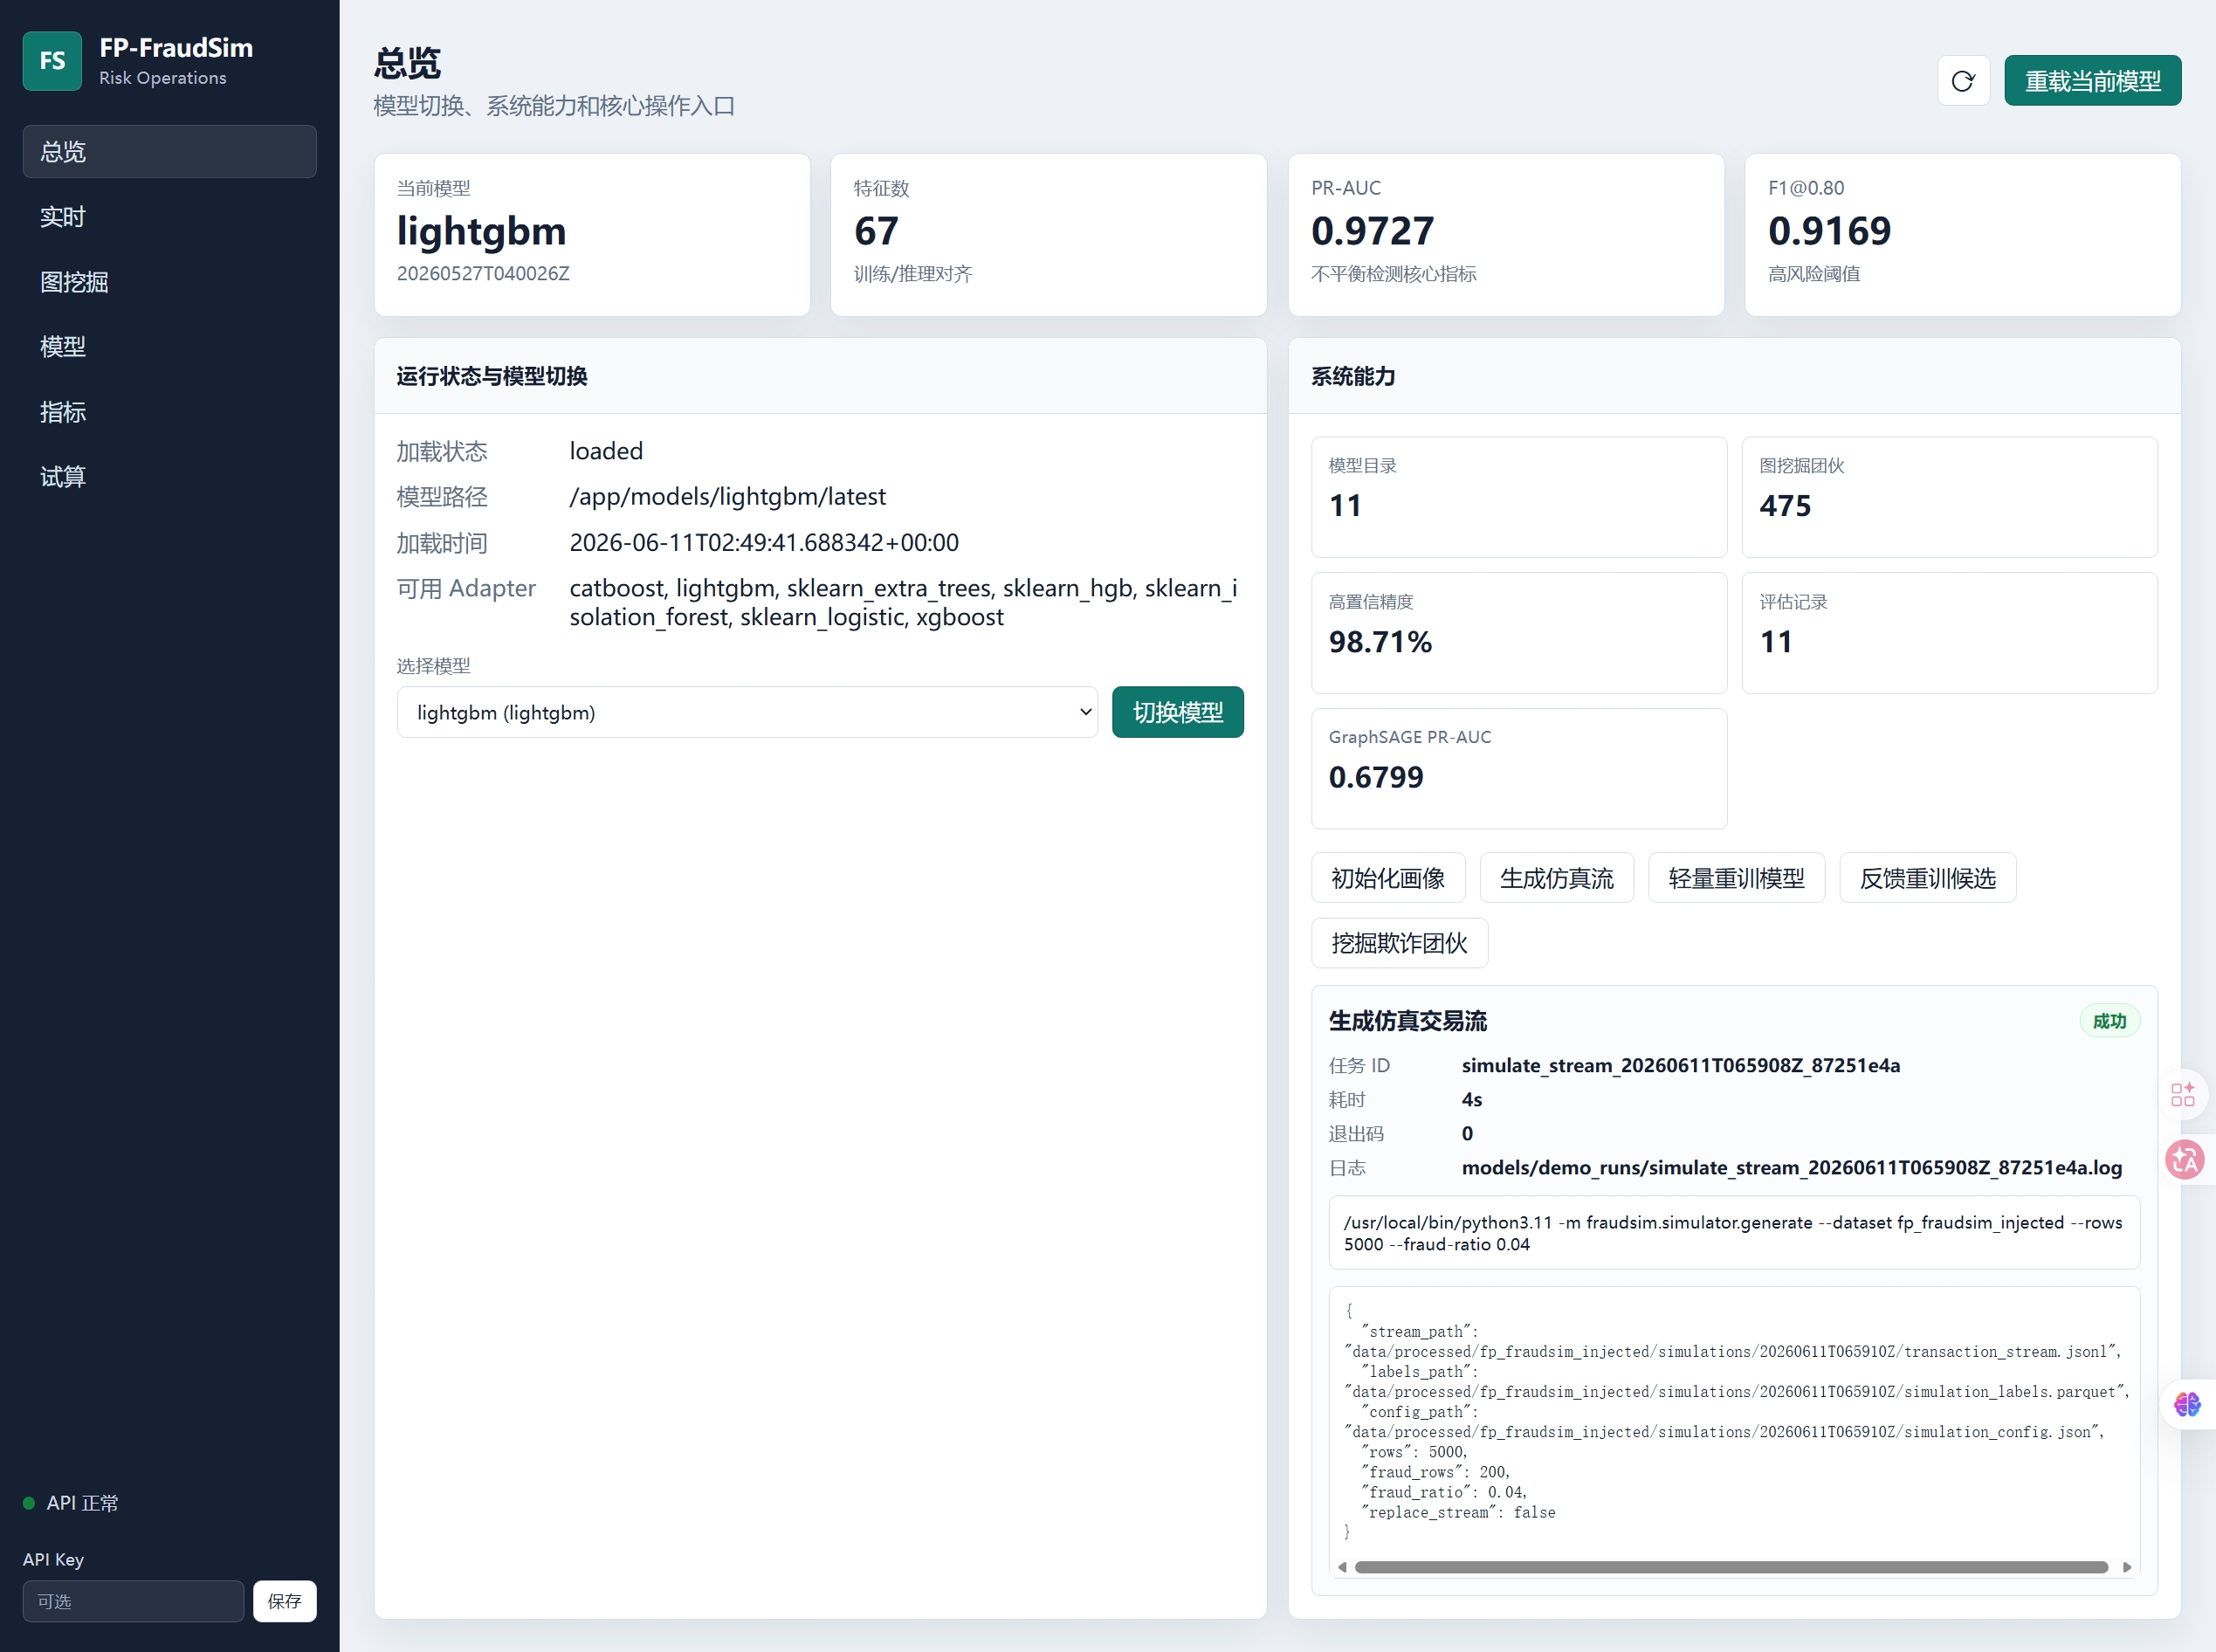
\includegraphics[width=0.92\textwidth]{pic/dashboard_overview_report.png}
  \caption{系统总览、服务状态与实时任务入口}
\end{figure}

\begin{figure}[H]
  \centering
  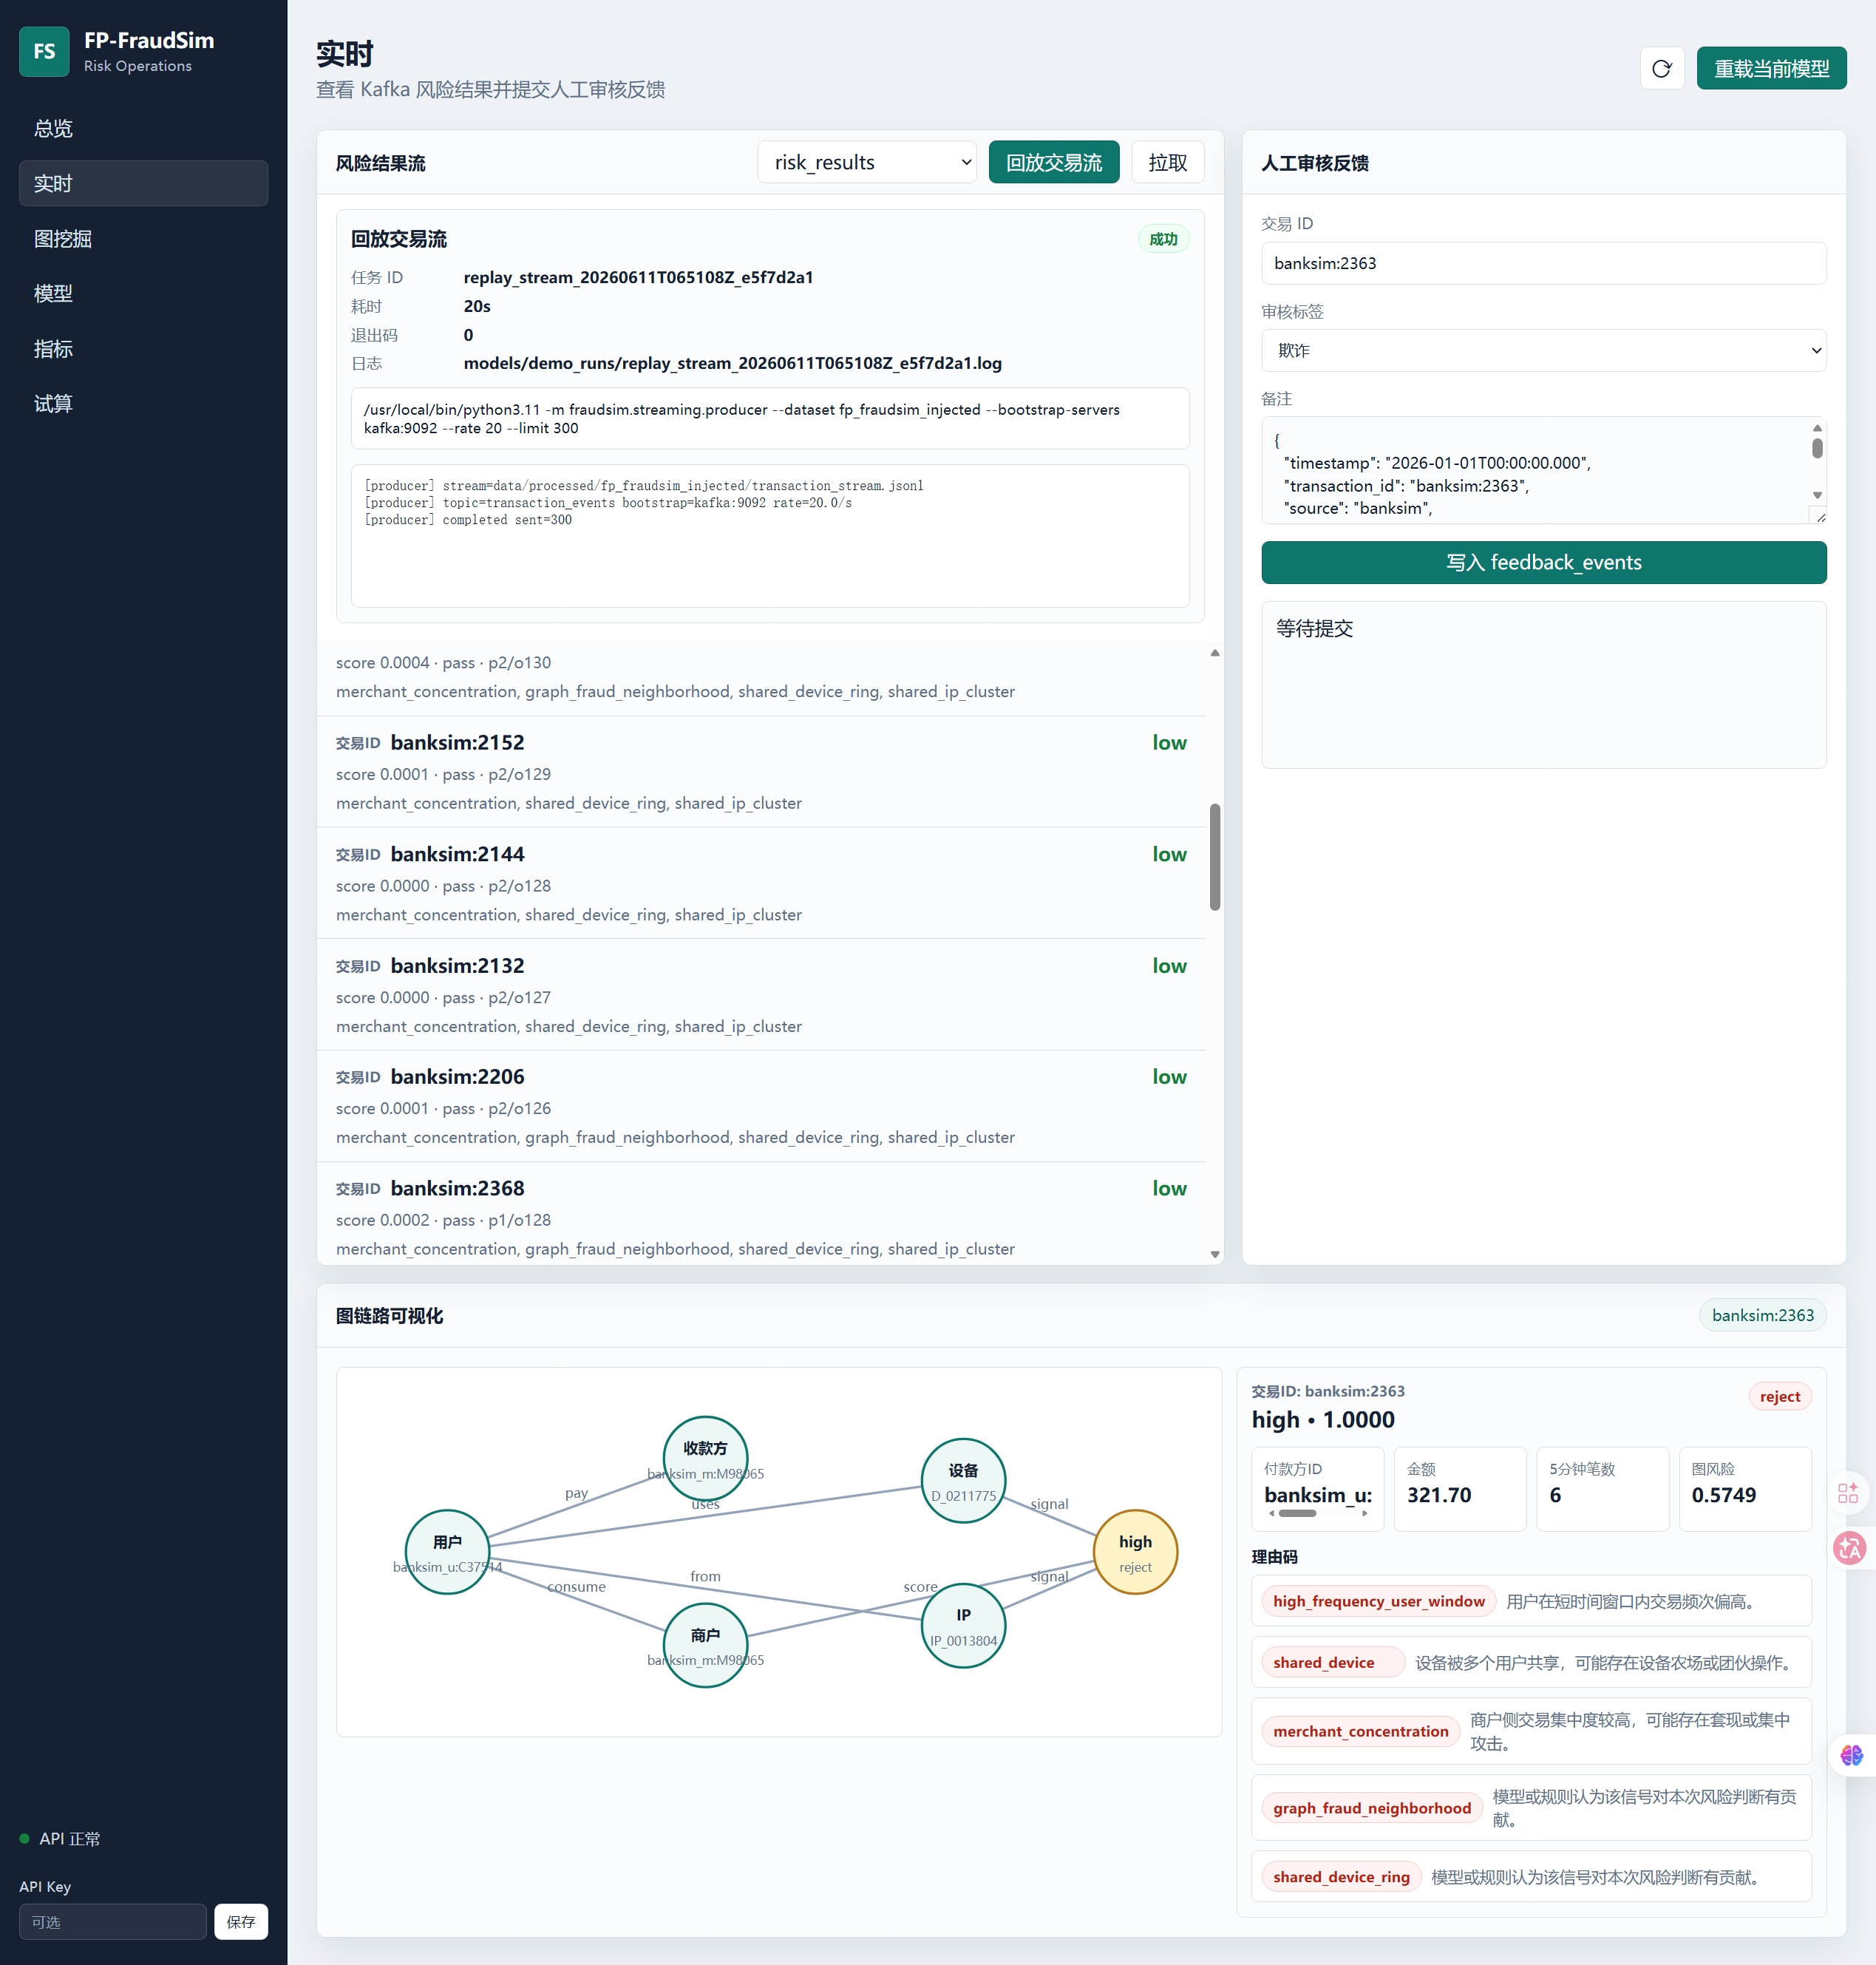
\includegraphics[width=0.82\textwidth]{pic/dashboard_replay_feedback_report.png}
  \caption{交易回放、风险结果与人工反馈闭环}
\end{figure}

\subsection{交付清单与复现保障}

项目交付包括代码工程、部署文件、测试、技术文档、指标报告和Dashboard。详细逐项交付清单见附录C；核心自动化测试覆盖如下。

\subsubsection{自动化测试覆盖}

项目包含面向核心模块的单元测试，除原有特征、窗口、微批、图挖掘和API测试外，新增可调仿真器、阈值沙盒、GraphSAGE数据构建和Kubernetes清单结构测试。

\begin{itemize}
  \item \code{test\_features.py}：验证训练特征选择、缺失填充和类别处理；
  \item \code{test\_window\_features.py}：验证用户、设备、IP、商户窗口统计；
  \item \code{test\_streaming\_microbatch.py}：验证微批评分缓冲与flush逻辑；
  \item \code{test\_graph\_mining\_explainability.py}：验证团伙挖掘和解释字段；
  \item \code{test\_api\_dashboard.py}：验证Dashboard资源、模型发现、指标和模型重载。
  \item \code{test\_simulator.py}与\code{test\_threshold\_sandbox.py}：验证仿真配置和阈值指标计算；
  \item \code{test\_graphsage\_experiment.py}与\code{test\_k8s\_manifests.py}：验证图采样、节点标签和边云资源清单。
\end{itemize}

测试运行命令为：

\begin{lstlisting}[language=bash]
python -m unittest discover -s tests
\end{lstlisting}

\section{创新性、实用性与安全设计}
\label{sec:conclusion}

\subsection{主要创新点}

\textbf{第一，系统级闭环而非单点模型。}本作品将欺诈样本注入、交易流回放、Flink实时计算、模型API、Dashboard展示、人工反馈和重训接口串联为闭环，能够直接演示“新增交易进入系统、实时评分、告警输出、人工复核、模型迭代”的完整过程，更贴近真实金融风控系统。

\textbf{第二，窗口特征与画像特征在线一致。}离线训练通过\code{add\_offline\_window\_features}构造窗口统计，在线Flink作业使用同一套\code{compute\_window\_feature\_dict}逻辑实时计算，降低训练/推理特征偏差。画像数据通过Redis按实体ID补齐，兼顾实时性和特征丰富度。

\textbf{第三，可解释图挖掘与GraphSAGE旁路并行。}系统围绕共享设备、IP、商户和收款方生成团伙证据链，同时以GraphSAGE旁路实验验证图嵌入价值。线上决策不直接使用未经充分验证的图嵌入，体现对创新探索与主链路稳定性的平衡。

\textbf{第四，阈值沙盒连接模型指标与业务研判。}模型分数被转换为风险等级、处置动作和理由码，阈值沙盒允许实时观察不同阈值下的精度、召回、误拦、漏过和审核工作量，使模型优化能够直接映射到业务成本。

\textbf{第五，微批推理提升工程可用性。}在线评分支持单笔与微批两种模式。微批模式通过批大小和等待时间控制延迟上界，在高并发流量下显著减少API调用次数，为后续横向扩展和生产化部署预留空间。

\textbf{第六，反馈驱动但受控发布。}系统采用candidate/latest/rollback三段式模型生命周期。反馈样本先训练候选模型，经指标核验和人工确认后发布，异常时可快速回滚，避免“自动学习”直接导致线上模型退化。

\subsection{实用性与业务适配}

本系统面向第三方支付交易风控，输出内容与业务处置流程一致：低风险交易放行，中风险交易人工复核，高风险交易拒绝并写入告警。Kafka主题天然适合接入上游支付网关和下游告警、审核、风控策略系统；FastAPI模型服务可独立扩容；Redis画像服务可替换为企业内部画像库或特征平台；Dashboard可作为比赛演示版，也可扩展为运营监控台。

在业务规则层面，系统覆盖常见反诈场景：异常大额、短时高频、多账户共设备、代理IP、风险商户集中、欺诈邻域和团伙命中。上述特征均可映射到真实金融机构风控经验，便于与规则引擎、黑名单、设备指纹系统和人工审核流程对接。

\subsection{成熟度与可扩展性}

代码结构按功能模块拆分，\code{fraudsim/models}负责模型适配，\code{fraudsim/training}负责训练，\code{fraudsim/streaming}负责流式链路，\code{fraudsim/api}负责服务接口，\code{fraudsim/dashboard}负责前端展示，\code{scripts}负责数据、启动和压测。新增模型只需实现统一适配器并注册；新增欺诈场景可在注入脚本中扩展；新增画像字段可通过特征配置自动进入训练与推理；新增下游系统可订阅Kafka输出主题。

系统提供Dockerfile、Dockerfile.flink、Dockerfile.graph和docker-compose.yml，使运行环境可复制；同时提供边缘实时侧与中心训练侧Kubernetes清单。边缘清单包含双副本Model API、Flink、Kafka、Redis、Secret和NetworkPolicy，中心清单包含候选模型训练与GraphSAGE实验CronJob。离线结构校验结果为20个资源有效、0个无效、0个错误。

\subsection{安全与合规设计}

金融反诈系统处理交易、设备、IP和账户行为数据，必须满足全生命周期安全要求。当前作品使用仿真与脱敏数据，并已实现部分基础安全能力：

\begin{enumerate}
  \item \textbf{数据最小化与脱敏：}训练和展示层仅使用实体ID哈希值，不展示姓名、证件号、手机号、银行卡号等直接身份标识；演示数据使用仿真样本；
  \item \textbf{敏感接口认证：}配置\code{FRAUDSIM\_API\_KEY}后，预测、反馈、重载、演示任务、模型发布和回滚等接口要求\code{X-API-Key}；
  \item \textbf{双通道审计：}敏感操作同时写入本地\code{audit.jsonl}和Kafka的\code{audit\_events}主题，Kafka不可用时仍保留本地审计；
  \item \textbf{模型发布保护：}候选模型发布前自动备份当前线上模型，支持快速回滚；
  \item \textbf{部署隔离：}Kubernetes清单使用Secret注入密钥，并通过NetworkPolicy限制Model API访问范围；
  \item \textbf{生产增强方向：}实际部署中还需启用TLS/SASL、OAuth2或mTLS、实体ID令牌化、对象存储加密、RBAC与不可篡改审计留存。
\end{enumerate}

\subsection{局限性与后续工作}

当前系统仍有三点需要继续增强。第一，代码仓库未包含大体积数据和模型产物，最终提交应附带可复现的数据准备说明与关键实验产物。第二，GraphSAGE当前仅完成受控旁路实验，后续需补充时间切分、消融实验和稳定性验证后再评估是否融合线上决策。第三，Kubernetes清单已完成结构校验但未在真实多节点集群部署，生产级环境仍需补齐镜像仓库、StorageClass、TLS/SASL、Ingress、RBAC和故障恢复压测。

总体来看，FP-FraudSim已经覆盖赛题一所要求的主要技术面：能够按参数模拟跨时段、跨渠道与团伙欺诈交易，能够在Kafka + Flink链路中实时检测并输出风险等级，能够通过图证据、理由码与阈值沙盒辅助研判，并通过反馈样本、候选发布、审计和回滚形成受控迭代闭环。


\clearpage
\section*{\centering\heiti\zihao{4}参考文献}
\addcontentsline{toc}{section}{参考文献}
\begin{thebibliography}{99}

\bibitem{flink}
Apache Software Foundation.
\textit{Apache Flink Documentation}.
https://nightlies.apache.org/flink/

\bibitem{kafka}
Apache Software Foundation.
\textit{Apache Kafka Documentation}.
https://kafka.apache.org/documentation/

\bibitem{redis}
Redis Ltd.
\textit{Redis Documentation}.
https://redis.io/docs/

\bibitem{fastapi}
FastAPI.
\textit{FastAPI Documentation}.
https://fastapi.tiangolo.com/

\bibitem{lightgbm}
Ke, G., Meng, Q., Finley, T., Wang, T., Chen, W., Ma, W., Ye, Q., \& Liu, T.-Y. (2017).
LightGBM: A highly efficient gradient boosting decision tree.
\textit{Advances in Neural Information Processing Systems}, 30.

\bibitem{xgboost}
Chen, T., \& Guestrin, C. (2016).
XGBoost: A scalable tree boosting system.
\textit{Proceedings of the 22nd ACM SIGKDD International Conference on Knowledge Discovery and Data Mining}, 785--794.

\bibitem{catboost}
Prokhorenkova, L., Gusev, G., Vorobev, A., Dorogush, A. V., \& Gulin, A. (2018).
CatBoost: unbiased boosting with categorical features.
\textit{Advances in Neural Information Processing Systems}, 31.

\bibitem{graphsage}
Hamilton, W. L., Ying, R., \& Leskovec, J. (2017).
Inductive representation learning on large graphs.
\textit{Advances in Neural Information Processing Systems}, 30.

\bibitem{auc}
Davis, J., \& Goadrich, M. (2006).
The relationship between Precision-Recall and ROC curves.
\textit{Proceedings of the 23rd International Conference on Machine Learning}, 233--240.

\bibitem{paysim}
Lopez-Rojas, E. A., Elmir, A., \& Axelsson, S. (2016).
PaySim: A financial mobile money simulator for fraud detection.
\textit{Proceedings of the 28th European Modeling and Simulation Symposium}.

\bibitem{banksim}
Lopez-Rojas, E. A., \& Axelsson, S. (2014).
BankSim: A bank payments simulator for fraud detection research.
\textit{Proceedings of the 26th European Modeling and Simulation Symposium}.

\bibitem{ieeecis}
IEEE Computational Intelligence Society.
\textit{IEEE-CIS Fraud Detection}.
Kaggle Competition, 2019.

\bibitem{creditcard}
Dal Pozzolo, A., Caelen, O., Johnson, R. A., \& Bontempi, G. (2015).
Calibrating probability with undersampling for unbalanced classification.
\textit{2015 IEEE Symposium Series on Computational Intelligence}, 159--166.

\bibitem{elliptic}
Weber, M., Domeniconi, G., Chen, J., Weidele, D. K. I., Bellei, C., Robinson, T., \& Leiserson, C. E. (2019).
Anti-money laundering in Bitcoin: Experimenting with graph convolutional networks for financial forensics.
\textit{KDD Workshop on Anomaly Detection in Finance}.

\bibitem{dgraphfin}
Huang, X., et al. (2022).
DGraph: A large-scale financial dataset for graph anomaly detection.
\textit{Advances in Neural Information Processing Systems}, 35.

\bibitem{samld}
Oztas, B., et al. (2023).
SAML-D: Synthetic anti-money laundering transaction data.
\textit{Data in Brief}, 47.

\bibitem{amlsim}
IBM Research.
\textit{AMLSim: Anti-Money Laundering Simulator}.
https://github.com/IBM/AMLSim

\bibitem{docker}
Docker Inc.
\textit{Docker Compose Documentation}.
https://docs.docker.com/compose/

\end{thebibliography}


\clearpage
\section*{\centering\heiti\zihao{4}附\quad 录}
\addcontentsline{toc}{section}{附录}

{\songti\zihao{-4}
附录补充项目目录、核心命令和提交材料检查表，便于评审复现。

\subsection*{附录A 项目目录说明}

\renewcommand\arraystretch{1.0}
\begin{table}[H]
  \centering
  \caption{项目目录与功能}
  \renewcommand\arraystretch{1.3}
  \setlength{\tabcolsep}{5pt}
  \begin{tabularx}{0.95\textwidth}{>{\raggedright\arraybackslash}p{4.6cm}>{\raggedright\arraybackslash}X}
    \toprule
    路径 & 功能 \\
    \midrule
    \texttt{fraudsim/features.py} & 交易、用户、设备、IP、商户画像合并与训练特征选择。 \\
    \texttt{fraudsim/window\_features.py} & 离线和在线共享的滑动窗口特征计算。 \\
    \texttt{fraudsim/training/train.py} & 多模型训练、阈值校准、指标输出和排行榜更新。 \\
    \texttt{fraudsim/streaming/flink\_job.py} & Flink实时评分作业，输出风险、告警和迟到事件。 \\
    \texttt{fraudsim/api/app.py} & FastAPI模型服务、Dashboard接口、模型热切换、反馈和图挖掘接口。 \\
    \texttt{fraudsim/graph\_mining.py} & 疑似欺诈团伙挖掘、实体风险特征和证据链生成。 \\
    \texttt{fraudsim/dashboard/} & HTML、CSS、JavaScript实现的可视化看板。 \\
    \texttt{scripts/scripts/etl/} & 数据规范化、统一数据集构建、校验和欺诈模式注入。 \\
    \texttt{scripts/benchmark\_api\_latency.py} & 单笔和批量模型API延迟压测。 \\
    \texttt{tests/} & API、特征、窗口、流式微批和图解释单元测试。 \\
    \bottomrule
  \end{tabularx}
\end{table}

\subsection*{附录B 一键演示命令}

\begin{lstlisting}[language=bash]
# 训练模型
python -m fraudsim.training.train --dataset fp_fraudsim_injected --model lightgbm

# 启动基础服务和Flink风险作业
docker compose -p fraudsim up -d --build kafka redis model-api flink-jobmanager flink-taskmanager flink-risk-job

# 创建主题、加载画像、回放交易流
python -m fraudsim.streaming.topics --bootstrap-servers localhost:9094
python -m fraudsim.streaming.load_profiles --dataset fp_fraudsim_injected --redis-url redis://localhost:6379/0
python -m fraudsim.streaming.producer --dataset fp_fraudsim_injected --bootstrap-servers localhost:9094 --rate 100 --limit 1000

# 打开看板
http://localhost:8000/dashboard
\end{lstlisting}

\subsection*{附录C 评分材料检查表}

\begin{table}[H]
  \centering
  \caption{赛题一提交材料检查表}
  \renewcommand\arraystretch{1.3}
  \setlength{\tabcolsep}{5pt}
  \begin{tabularx}{0.95\textwidth}{>{\raggedright\arraybackslash}p{2.5cm}>{\raggedright\arraybackslash}X}
    \toprule
    检查项 & 说明 \\
    \midrule
    技术文档 & 本报告已覆盖任务理解、数据、特征、架构、模型、实验、安全和复现。 \\
    代码工程 & 根目录包含README、Dockerfile、docker-compose、训练、流式、API、Dashboard和测试代码。 \\
    数据与模型 & 大体积目录默认不入库，最终提交前应按赛事要求附带可复现数据包或下载/生成说明。 \\
    指标报告 & 由\texttt{metrics.json}、\texttt{leaderboard.json}和API延迟报告提供。 \\
    演示材料 & Dashboard可展示实时风险、告警、理由码、图团伙和人工反馈闭环。 \\
    安全说明 & 正文第五节给出脱敏、加密、权限、审计、模型安全和容器隔离设计。 \\
    \bottomrule
  \end{tabularx}
\end{table}
}


\clearpage
\section*{\centering\heiti\zihao{4}致\quad 谢}
\addcontentsline{toc}{section}{致谢}

{\songti\zihao{-4}
本文档在金融反诈智能守护赛题规则的基础上完成，感谢赛事组委会提供明确的任务方向和评价准则，使作品能够围绕真实金融风控场景进行系统化设计。

项目实现过程中参考了Kafka、Flink、Redis、FastAPI、Docker Compose以及LightGBM、XGBoost、CatBoost等开源项目文档和社区实践。上述开源生态为流式计算、模型服务、容器化部署和机器学习训练提供了稳定基础。

本文档不包含学校、指导教师姓名等可能违反赛事匿名要求的信息。作品仍有不足之处，敬请专家评委批评指正。
}



\end{document}
